% \documentclass[12pt,a4paper,oneside]{book}
% \usepackage[utf8]{vietnam}
% \usepackage{graphicx}
% \graphicspath{{images/}}
% \usepackage{appendix}
% \usepackage{listings}
% \usepackage{xcolor}
% \usepackage[linesnumbered,lined,ruled]{algorithm2e}

% \usepackage{etoolbox}

% \usepackage[unicode]{hyperref}

% \usepackage{setting/bkthesis}

% \usepackage[vietnamese]{babel}
% \usepackage{titlesec}
% \usepackage{titletoc}
% \usepackage{listings}


% %code hight light
% \lstset{frame=tb,
%   language=Java,
%   aboveskip=3mm,
%   belowskip=3mm,
%   showstringspaces=false,
%   columns=flexible,
%   basicstyle={\small\ttfamily},
%   numbers=left,
%   numberstyle=\tiny\color{gray},
%   keywordstyle=\color{blue},
%   commentstyle=\color{dkgreen},
%   stringstyle=\color{mauve},
%   breaklines=true,
%   breakatwhitespace=true,
%   tabsize=3,
%   float=H
% }

% \usepackage[left=3cm,right=2cm,top=2.5cm,bottom=3cm]{geometry}
% \usepackage{fancyhdr}
% \pagestyle{fancy}
% \fancyhead{}
% \fancyhead[RO,LE]{Thesis Title}
% \fancyfoot{}
% \fancyfoot[LE,RO]{\thepage}
% \fancyfoot[LO,CE]{Chapter \thechapter}
% \fancyfoot[CO,RE]{Author Name}

\documentclass[13pt,a4paper,oneside]{book} % twoside for draf

\usepackage[justification=centering]{caption}
%\usepackage{babel}
\usepackage[utf8]{vietnam}
\usepackage[vietnamese=nohyphenation]{hyphsubst}
%\usepackage{times}
%\usepackage{graphicx}

\usepackage{mathptmx}	% same Time New Roma
\usepackage{dirtytalk}
\usepackage{indentfirst}

%\renewcommand{\rmdefault}{phv} % Arial
%\renewcommand{\sfdefault}{phv} % Arial
% \usepackage[fontsize=13pt]{scrextend}
\usepackage[multiple]{footmisc}
\usepackage{fancyhdr}
% \usepackage[utf8]{inputenc}
\usepackage[vietnamese, english]{babel}
\usepackage{titlesec}
\usepackage{titletoc}
\usepackage{listings}
\usepackage[bookmarks=true]{hyperref}
\usepackage[left=3cm,right=2cm,top=2.5cm,bottom=3cm]{geometry}
\usepackage{graphicx}
\usepackage{hyperref}
\usepackage{tikz}
\usepackage{varwidth}
\usepackage{float}
\usepackage{color}
\usepackage{multirow}
\usepackage{booktabs}
\usepackage[linesnumbered,lined,ruled,resetcount, algochapter]{algorithm2e}
\usepackage{svg}
\usepackage{tabularx}
\usepackage{nomencl}
\usepackage{scrfontsizes}
\usepackage{longtable}
\usepackage{multicol}
\usepackage[toc,page]{appendix}
\usepackage{adjustbox}

\usepackage{makecell}
\usepackage{longtable}
\usepackage{multirow}
% \usepackage{algpseudocode}
\usepackage{setting/bkthesis}
\usepackage[toc]{appendix}
\usepackage{subcaption}
\usepackage{csquotes}
%\counterwithin{figure}{chapter}
\usepackage[
defernumbers,
sortcites,
backend=biber,
bibstyle=authoryear,
sorting=nyt,
citestyle=numeric-comp
]{biblatex}
\usepackage{xpatch}

\makeatletter
\input{numeric.bbx}
\makeatother

\xpatchbibmacro{date+extrayear}{%
  \printtext[parens]%
}{%
  \setunit{\addperiod\space}%
  \printtext%
}{}{}

% \usepackage{biblatex}
\addbibresource{refs.bib}

% \renewcommand\labelitemi{--}

\setlength{\parskip}{6pt}

\usetikzlibrary{calc}
\setlength{\parindent}{10mm}
\renewcommand{\baselinestretch}{1.3}
\graphicspath{{images/}}
\renewcommand{\listalgorithmcfname}{Danh sách thuật toán}
\renewcommand{\nomname}{Danh sách ký hiệu, viết tắt}
\renewcommand\appendixtocname{Phụ lục}

\SetKwRepeat{Do}{do}{while}%

\usepackage{tikz}
\usetikzlibrary{shapes.geometric}
\usetikzlibrary{arrows.meta,arrows}

% \algdef{SE}[DOWHILE]{Do}{doWhile}{\algorithmicdo}[1]{\algorithmicwhile\ #1}%
% \usepackage{setting/uetthesis}

%%% The following lines add Chapter or Appendix in front of the number
\titlecontents{chapter}%
[0pt]%
{\vspace{1ex}}%
{\bfseries Chương \thecontentslabel\quad}%
{\bfseries}%
{\bfseries\hfill\contentspage}
%%% Initially, for the main part of the document, set the label to "Chapter"
\let\chapappname\chaptername

\setcounter{tocdepth}{4}
\setcounter{secnumdepth}{4}

% \thesislayout
% hyper setup
\definecolor{dkgreen}{rgb}{0,0.6,0}
\definecolor{gray}{rgb}{0.5,0.5,0.5}
\definecolor{mauve}{rgb}{0.58,0,0.82}

% setup code area as listings
\lstset{frame=tb,
  language=Java,
  xleftmargin=10pt,xrightmargin=10pt,
%   framesep=2cm,
%   aboveskip=2cm,
%   belowskip=2cm,
  showstringspaces=false,
  columns=flexible,
  basicstyle={\small\ttfamily},
  numbers=left,
  numberstyle=\tiny\color{gray},
  keywordstyle=\color{blue},
  commentstyle=\color{dkgreen},
  stringstyle=\color{mauve},
  breaklines=true,
  breakatwhitespace=true,
  tabsize=2
}

\renewcommand{\bibname}{Whatever floats your boat}

\newcommand{\tcode}[1]{{\ttfamily\selectfont#1}}

\hypersetup{
	bookmarks=true,
	pdftitle={DEVELOP A MANAGEMENT SYSTEM FOR SMALL AND MEDIUM-SIZED EATERIES},
	pdfauthor={Trần Tuấn Thịnh}, % author
	pdfsubject={centralized platform},
	pdfkeywords={TeX, LaTeX, graphics, images, thesis, restaurants}, % list of keywords
	colorlinks=false,       % false: boxed links; true: colored links
	linkcolor=black,       % color of internal links
	citecolor=black,       % color of links to bibliography
	filecolor=black,        % color of file links
	urlcolor=black,        % color of external links
	linktoc=page           % only page is linked
}

\colorlet{punct}{red!60!black}
\definecolor{delim}{RGB}{20,105,176}
\colorlet{numb}{magenta!60!black}
\lstdefinelanguage{json}{
    basicstyle=\normalfont\ttfamily,
    numbers=left,
    numberstyle=\scriptsize,
    stepnumber=1,
    numbersep=8pt,
    showstringspaces=false,
    breaklines=true,
    frame=lines,
    literate=
     *{0}{{{\color{numb}0}}}{1}
      {1}{{{\color{numb}1}}}{1}
      {2}{{{\color{numb}2}}}{1}
      {3}{{{\color{numb}3}}}{1}
      {4}{{{\color{numb}4}}}{1}
      {5}{{{\color{numb}5}}}{1}
      {6}{{{\color{numb}6}}}{1}
      {7}{{{\color{numb}7}}}{1}
      {8}{{{\color{numb}8}}}{1}
      {9}{{{\color{numb}9}}}{1}
      {:}{{{\color{punct}{:}}}}{1}
      {,}{{{\color{punct}{,}}}}{1}
      {\{}{{{\color{delim}{\{}}}}{1}
      {\}}{{{\color{delim}{\}}}}}{1}
      {[}{{{\color{delim}{[}}}}{1}
      {]}{{{\color{delim}{]}}}}{1},
}


\lstdefinelanguage{JavaScript}{
  morekeywords=[1]{break, continue, delete, else, for, function, if, in,
    new, return, this, typeof, var, void, while, with},
  % Literals, primitive types, and reference types.
  morekeywords=[2]{false, null, true, boolean, number, undefined,
    Array, Boolean, Date, Math, Number, String, Object},
  % Built-ins.
  morekeywords=[3]{eval, parseInt, parseFloat, escape, unescape},
  sensitive,
  morecomment=[s]{/*}{*/},
  morecomment=[l]//,
  morecomment=[s]{/**}{*/}, % JavaDoc style comments
  morestring=[b]',
  morestring=[b]"
}[keywords, comments, strings]

\lstalias[]{ES6}[ECMAScript2015]{JavaScript}

\lstdefinelanguage[ECMAScript2015]{JavaScript}[]{JavaScript}{
  morekeywords=[1]{await, async, case, catch, class, const, default, do,
    enum, export, extends, finally, from, implements, import, instanceof,
    let, static, super, switch, throw, try},
  morestring=[b]` % Interpolation strings.
}
\renewcommand\autoref[1]{%
	\hyperref[#1]{\ref*{#1}}%
}
\renewcommand*{\algorithmcfname}{Thuật toán}
\renewcommand\lstlistlistingname{Danh sách đoạn mã}
\renewcommand{\lstlistingname}{Đoạn mã}
\makeatletter
\renewcommand\@seccntformat[1]{\csname the#1\endcsname.\quad}
\makeatother
% \renewcommand\thechapter{\arabic{chapter}}
%\renewcommand\thesection{\thechapter.\arabic{section}.}
%\renewcommand\thesubsection{\thesection\arabic{subsection}.}
%\renewcommand\thesubsubsection{\thesubsection\arabic{subsubsection}.}
\renewcommand{\thetable}{\thechapter.\arabic{table}}
\renewcommand{\thefigure}{\thechapter.\arabic{figure}}
\renewcommand{\thealgocf}{\thechapter.\arabic{algocf}}

\newcolumntype{R}{>{\raggedleft\arraybackslash}X}
\newcolumntype{L}{>{\raggedright\arraybackslash}X}
\newcolumntype{F}[1]{>{\raggedleft\let\newline\\\arraybackslash\hspace{0pt}}m{#1}}

\let\oldFootnote\footnote
\newcommand\nextToken\relax

\renewcommand\footnote[1]{%
	\oldFootnote{#1}\futurelet\nextToken\isFootnote}

\newcommand\isFootnote{%
	\ifx\footnote\nextToken\textsuperscript{,}\fi}

\begin{document}
\renewcommand{\thelstlisting}{\thechapter.\arabic{lstlisting}}

\pagestyle{plain}
\frontmatter

%-------TITLE PAGE------%
\begin{titlepage}
	\center
	\begin{tikzpicture}[overlay,remember picture]
		\draw [line width=3pt,rounded corners=0pt,]
		($ (current page.north west) + (25mm,-25mm) $)
		rectangle
		($ (current page.south east) + (-15mm,25mm) $);
		\draw [line width=1pt,rounded corners=0pt]
		($ (current page.north west) + (26.5mm,-26.5mm) $)
		rectangle
		($ (current page.south east) + (-16.5mm,26.5mm) $);
	\end{tikzpicture}
	
	{\large \bfseries ĐẠI HỌC QUỐC GIA HÀ NỘI\\ TRƯỜNG ĐẠI HỌC CÔNG NGHỆ}\\[1cm]
	\includesvg[width=0.25\linewidth]{images/Logo_HUET.svg}\\[1cm]
	{\Large  \bfseries Trần Tuấn Thịnh}\\[1.5cm]
	{ \LARGE \bfseries  PHÁT TRIỂN HỆ THỐNG }\\[0.2cm]
    {\LARGE \bfseries HỖ TRỢ QUẢN LÝ NHÀ HÀNG VỪA VÀ NHỎ}\\[0.2cm]
     % { \LARGE \bfseries CHUYÊN NGHIỆP HÓA NGÀNH DỊCH VỤ ĂN UỐNG}\\[0.2cm]
	\hfill\\[2cm]
	{\large \bfseries KHÓA LUẬN TỐT NGHIỆP ĐẠI HỌC HỆ CHÍNH QUY}\\	
	{\large \bfseries Ngành: Công nghệ thông tin}	
	\hfill\\[5.3cm]	
	{\large \bfseries HÀ NỘI - 2024}\\	
	\vfill
\end{titlepage}

%-------TITLE PAGE+6hbk,------%
\begin{titlepage}
	\center
	\begin{tikzpicture}[overlay,remember picture]
	\draw [line width=3pt,rounded corners=0pt,]
	($ (current page.north west) + (25mm,-25mm) $)
	rectangle
	($ (current page.south east) + (-15mm,25mm) $);
	\draw [line width=1pt,rounded corners=0pt]
	($ (current page.north west) + (26.5mm,-26.5mm) $)
	rectangle
	($ (current page.south east) + (-16.5mm,26.5mm) $);
	\end{tikzpicture}
	
	{\large \bfseries ĐẠI HỌC QUỐC GIA HÀ NỘI\\ TRƯỜNG ĐẠI HỌC CÔNG NGHỆ}\\[2cm]
% 	\includegraphics[width=0.25\linewidth]{images/Logo_UET.png}\\[1cm]
	
	{\Large  \bfseries Trần Tuấn Thịnh}\\[2cm]		
	{ \LARGE \bfseries  PHÁT TRIỂN HỆ THỐNG }\\[0.2cm]
    {\LARGE \bfseries HỖ TRỢ QUẢN LÝ NHÀ HÀNG VỪA VÀ NHỎ}\\[0.2cm]
     % { \LARGE \bfseries CHUYÊN NGHIỆP HÓA NGÀNH DỊCH VỤ ĂN UỐNG}\\[0.2cm]
	\hfill\\[1.5cm]
	{\large \bfseries KHÓA LUẬN TỐT NGHIỆP ĐẠI HỌC HỆ CHÍNH QUY}\\	
	{\large \bfseries Ngành: Công nghệ thông tin}
	\hfill\\[2cm]
	\begin{flushleft}
	    	{\large \bfseries Cán bộ hướng dẫn: TS. Võ Đình Hiếu}\\
	\end{flushleft}
	\hfill\\[2.5cm]	
	\begin{flushleft}
% 	{\large \bfseries Cán bộ đồng hướng dẫn: CN. Bùi Quang Cường}\\	
	\end{flushleft}
		\hfill\\[3cm]	
	{\large \bfseries HÀ NỘI - 2024}\\		
	\vfill		
\end{titlepage}

%-------TITLE PAGE+6hbk,------%
\begin{titlepage}
	\center
	\begin{tikzpicture}[overlay,remember picture]
	\draw [line width=3pt,rounded corners=0pt,]
	($ (current page.north west) + (25mm,-25mm) $)
	rectangle
	($ (current page.south east) + (-15mm,25mm) $);
	\draw [line width=1pt,rounded corners=0pt]
	($ (current page.north west) + (26.5mm,-26.5mm) $)
	rectangle
	($ (current page.south east) + (-16.5mm,26.5mm) $);
	\end{tikzpicture}
	
	{\large \bfseries VIETNAM NATIONAL UNIVERSITY, HANOI\\ UNIVERSITY OF ENGINEERING AND TECHNOLOGY}\\[2cm]
% 	\includegraphics[width=0.25\linewidth]{images/Logo_UET.png}\\[1cm]
	
	{\Large  \bfseries Tran Tuan Thinh}\\[2cm]	
 % Develop a management system for small and medium-sized restaurants
	{ \LARGE \bfseries DEVELOP A MANAGEMENT SYSTEM }\\[0.2cm] 
	{\LARGE \bfseries FOR SMALL AND MEDIUM-SIZED EATERIES }\\[0.2cm]
    % {\LARGE \bfseries PROFESSIONALIZE THE FOOD SERVICE INDUSTRY }\\[0.2cm]
	\hfill\\[1.5cm]
	{\large \bfseries BACHELOR’S THESIS}\\	
	{\large \bfseries Major: Information Technology}
	\hfill\\[2cm]
	\begin{flushleft}
	    	{\large \bfseries Supervisor: Dr. Vo Dinh Hieu}\\
	\end{flushleft}
	\hfill\\[2.5cm]	
	\begin{flushleft}
% 	{\large \bfseries Cán bộ đồng hướng dẫn: CN. Bùi Quang Cường}\\	
	\end{flushleft}
		\hfill\\[3cm]	
	{\large \bfseries Hanoi - 2024}\\
	\vfill		
\end{titlepage}

\changefontsizes[16pt]{13pt}
\addtocontents{toc}{\vspace{-1cm}}
\addcontentsline{toc}{chapter}{Lời cam đoan}
\begin{center}
    \textbf{LỜI CAM ĐOAN}
\end{center}

% Em xin cam đoan: Khóa luận tốt nghiệp với đề tài “Phát triển hệ sinh thái hỗ trợ quán ăn và thực khách giúp chuyên nghiệp hóa ngành dịch vụ ăn uống” trong báo cáo này là của em.
% Những gì em viết ra không có sự sao chép từ các tài liệu, không sử dụng kết quả của người khác mà không trích dẫn cụ thể.
% Đây là công trình nghiên cứu cá nhân em tự phát triển, không sao chép mã nguồn của người khác.
% Nếu vi phạm những điều trên, em xin chấp nhận tất cả những truy cứu về trách nhiệm theo quy định của Trường Đại học Công nghệ - ĐHQGHN.

Tôi tên là Trần Tuấn Thịnh, sinh viên của lớp QH-2020-I/CQ-C-CLC, ngành Công nghệ thông tin hệ chất lượng cao.
Tôi xin cam đoan rằng đề tài khóa luận tốt nghiệp của tôi với chủ đề \say{Phát triển hệ thống hỗ trợ quản lý nhà hàng vừa và nhỏ} là sản phẩm nghiên cứu của bản thân tôi và chưa bao giờ được nộp làm khóa luận tốt nghiệp cho bất kỳ trường đại học nào, trong đó có Trường Đại học Công nghệ.
Tôi cam đoan rằng tôi không sao chép bất kỳ nội dung nào từ các tài liệu khác, cũng như không sử dụng kết quả của bất kỳ người nào khác mà không có trích dẫn cụ thể.
Đây là công trình nghiên cứu do cá nhân tôi thực hiện với sự hướng dẫn của TS Võ Đình Hiếu, không chứa bất kỳ mã nguồn nào được sao chép, chỉnh sửa từ cá nhân, tổ chức nào khác mà không được cho phép.
Nếu vi phạm những điều trên, tôi hoàn toàn chấp nhận mọi trách nhiệm theo quy định của Trường Đại học Công nghệ.

\begin{flushright}
	\begin{varwidth}{\linewidth}\centering
		Hà Nội, ngày 27 tháng 5 năm 2024\\
		Sinh viên\\[2cm]
		Trần Tuấn Thịnh
	\end{varwidth}
\end{flushright}

\newpage

\addcontentsline{toc}{chapter}{Lời cảm ơn}
\begin{center}
    \textbf{LỜI CẢM ƠN}
\end{center}

Lời đầu tiên cho phép em được gửi lời cảm ơn tới Khoa Công Nghệ Thông Tin – Trường Đại học Công nghệ - ĐHQG Hà Nội đã tạo điều kiện thuận lợi cho em được học tập, nghiên cứu và thực hiện đề tài tốt nghiệp này.

Em cũng xin được bày tỏ lòng biết ơn sâu sắc tới thầy Võ Đình Hiếu đã tận tình hướng dẫn, đóng góp những ý kiến xác đáng để em có thể hoàn thành khóa luận một cách tốt nhất.
Thời gian được làm việc và nghiên cứu tại phòng thí nghiệm thật sự đã đem lại những kinh nghiệm, những kiến thức quý báu và vô giá đối với bản thân em.

Cuối cùng, em cũng vô cùng biết ơn những thầy cô trong trường đã tận tình giảng dạy, trang bị cho em những kiến thức quan trọng để em có đầy đủ kiến thức và kỹ năng để có thể tự tin đi tiếp những chặng đường tiếp theo.

Chúc mọi người luôn luôn vui vẻ và gặt hái được nhiều thành công trong cuộc sống.

\newpage
\addcontentsline{toc}{chapter}{Tóm tắt}
\begin{center}
    \textbf{TÓM TẮT}
\end{center}
\changefontsizes[16pt]{12pt}
\textit{\textbf{Tóm tắt: }} 
Khóa luận trình bày về quá trình phát triển một nền tảng tập trung hỗ trợ quản lý nhà hàng và hỗ trợ đặt đồ ăn dành riêng cho các nhà hàng vừa và nhỏ.

Hệ thống này sẽ cung cấp một ứng dụng quản lý cho một doanh nghiệp với các chức năng đầy đủ và toàn diện như quản lý bán hàng, doanh thu, nhân viên, khách hàng cũng như hỗ trợ quảng bá cho nhà hàng.
Điều này giúp tối ưu hóa hoạt động kinh doanh của nhà hàng, giúp giảm thiểu chi phí nhân viên và vận hành, quản lý.
Ngoài ra, hệ thống cũng tích hợp tính năng đặt đồ ăn thông qua quét mã QR với giao diện thân thiện, dễ sử dụng, cho phép khách hàng dễ dàng đặt món và thanh toán tại nhà hàng trên nền tảng.

Bằng việc áp dụng kiến trúc vi dịch vụ (microservice) khi phát triển và triển khai hệ thống, từng dịch vụ như thông báo, đặt đồ ăn, quản lý nhà hàng, v.v. sẽ được tách biệt riêng với nhau giúp tăng tính sẵn sàng cũng như là khả năng chịu lỗi của hệ thống.
Ngoài ra về sau khi số lượng người dùng tăng, kiến trúc này cũng đảm bảo khả năng nâng cấp linh hoạt, dễ dàng và đặc biệt trong những khung giờ cao điểm khi số lượng người dùng vượt quá mức sử dụng thường thấy, hệ thống hoàn toàn có thể tự động mở rộng mà không cần tới sự can thiệp của quản trị viên hệ thống.
\vspace{-0.5cm}
\begin{flushleft}
  \textit{\textbf{Từ khóa: } Microservice, tự động mở rộng, quản lý quán ăn, nhà hàng, nền tảng tập trung}
\end{flushleft}

\newpage
\addcontentsline{toc}{chapter}{Abstract}
\begin{center}
    \textbf{ABSTRACT}
\end{center}
\changefontsizes[16pt]{12pt}
\textit{\textbf{Abstract: }} 
This thesis presents the development process of a centralized system to support restaurant management and online food ordering specifically for small and medium-sized restaurants.

The system will provide a management application for businesses with comprehensive and full-fledged functionalities such as sales, revenue, staff, and customer management, as well as restaurant promotion support.
This will help optimize restaurant operations, minimize staff and operational costs, and management.
In addition, the system also integrates food ordering feature through QR scanning with a friendly and easy-to-use interface, allowing customers to easily order and pay for food at the restaurant on the platform.

By applying a microservice architecture to the development and deployment of the system, each service such as notifications, food ordering, restaurant management, etc., will be separated from each other, increasing the availability and fault tolerance of the system.
Additionally, as the number of users increases, this architecture also ensures flexible and easy upgradeability, and especially during peak hours when the number of users exceeds the usual usage, the system can automatically scale without the need for system administrator intervention.
\vspace{-0.5cm}
\begin{flushleft}
  \textit{\textbf{Keywords: } Microservice, auto-scaling, restaurant management, restaurants, centralized platform}
\end{flushleft}
\changefontsizes[16pt]{13pt}


\changefontsizes[16pt]{13pt}
% \input{chapters/0.2.start}

\renewcommand{\contentsname}{Mục lục}
\tableofcontents

% \pagestyle{fancy}

\renewcommand{\listfigurename}{Danh sách hình vẽ}
\addcontentsline{toc}{chapter}{\listfigurename}
\listoffigures

\renewcommand{\listtablename}{Danh sách bảng}
\listoftables
\addcontentsline{toc}{chapter}{\listtablename}

\listofalgorithms
\addcontentsline{toc}{chapter}{\listalgorithmcfname}

\lstlistoflistings
\addcontentsline{toc}{chapter}{\lstlistlistingname}

\renewcommand{\chaptername}{Chương}
\renewcommand{\figurename}{Hình}
\renewcommand{\tablename}{Bảng}

% \newpage
\chapter*{Thuật ngữ}
\addcontentsline{toc}{chapter}{Thuật ngữ}
\changefontsizes[16pt]{13pt}
\begin{table}[h!]
    \centering
\resizebox{\textwidth}{!}{%
	\begin{tabular}{|ll|l|}
		\hline
		\multicolumn{2}{|c|}{\textbf{Thuật ngữ}}                                             & \multicolumn{1}{c|}{\multirow{2}{*}{\textbf{Ý nghĩa}}} \\ \cline{1-2}
		\multicolumn{1}{|c|}{\textbf{Từ viết tắt}} & \multicolumn{1}{c|}{\textbf{Từ đầy đủ}} & \multicolumn{1}{c|}{}                                  \\ \hline
		\multicolumn{1}{|l|}{K8s}                  & Kubernetes                    & Cây cú pháp trừu tượng                                 \\ \hline
		\multicolumn{1}{|l|}{CSP}                  & Cloud Service Provider                      & Đồ thị dòng điều khiển                                 \\ \hline
		\multicolumn{1}{|l|}{GCP}                  & Google Cloud Platform                           & Dòng mã                                                \\ \hline
		\multicolumn{1}{|l|}{GKE}                 & Google Kubernetes Engine                & Ngôn ngữ đánh dấu siêu văn bản                         \\ \hline
		\multicolumn{1}{|l|}{HTML}                  & Hypertext Markup Language          & Lý thuyết mô-đun thỏa mãn                              \\ \hline
		\multicolumn{1}{|l|}{JSX}                  & JavaScript XML          & Lý thuyết mô-đun thỏa mãn                              \\ \hline
		\multicolumn{1}{|l|}{GLSB}                  & Global Server Load Balancers          & Lý thuyết mô-đun thỏa mãn                              \\ \hline
		\multicolumn{1}{|l|}{}                  & Microservice          & kiến trúc vi dịch vụ                              \\ \hline
		\multicolumn{1}{|l|}{}                  & Message Queue          & hàng đợi tin nhắn                              \\ \hline
		\multicolumn{1}{|l|}{}                  & API Gateway          & Cổng API                              \\ \hline
		\multicolumn{1}{|l|}{}                     & Request                                    & yêu cầu                                       \\ \hline
	\end{tabular}%
}
\end{table}
\mainmatter

\changefontsizes[16pt]{13pt}
\pagestyle{plain}
\chapter*{Đặt vấn đề}\label{chap0}
\addcontentsline{toc}{chapter}{Đặt vấn đề}
% \vspace{5mm}
% \begin{figure}[h]
% 	\begin{tabular}{cc}
% 		\begin{minipage}[b]{0.5\textwidth}
% 			\begin{lstlisting}[language=C++]
% class B {
% 	int b;
% 	int stub(int x); // ERROR
% }
% int foo(B param) {
% 	if (param.b == 1) {
% 		int ret = param.stub(b);
% 		if (param.b == 2) 
% 		return ret;
% 	}
% 	return 0; 
% }  
% 			\end{lstlisting}
% 		\end{minipage}
% 		& \begin{minipage}[b]{0.5\textwidth}
% 			\centering
% 			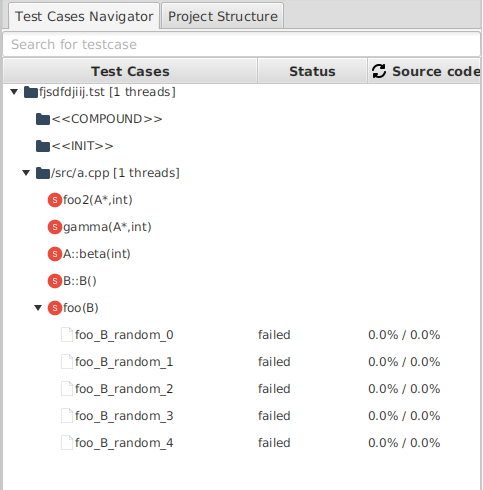
\includegraphics[width=\linewidth]{images/effect.png}
% 		\end{minipage}
% 	\end{tabular}
% 	\caption{Ví dụ sự ảnh hưởng của hàm thiếu định nghĩa khi kiểm thử đơn vị tự động.}
% 	\label{fig:affect}
% \end{figure}

Hiện nay, trong thời đại chuyển đối số khi mà mọi giao dịch, thanh toán đều được thực hiện trên thiết bị di động của người dùng, các nhà phát triển phần mềm đứng trước một cơ hội để tối ưu hóa các quy trình rườm rà đã có nhằm giảm thiểu tương tác trực tiếp giữa nhà cung cấp dịch vụ và người dùng từ đó đẩy nhanh quy trình nghiệp vụ.
Một trong các lĩnh vực được quan tâm và chuyển đổi mạnh mẽ trong những năm gần đây đó là về lĩnh vực dịch vụ ăn uống tại Việt Nam.
Trong đại dịch Covid-19, đã có một sự dịch chuyển lớn trong ngành ẩm thực.
Năm 2020, một khảo sát đã chỉ ra rằng số lượng người đến ăn tại nhà hàng đã giảm trên 90\% do lệnh phong tỏa của các quốc gia và nỗi sợ nguy cơ lây nhiễm từ người qua người~\cite{dube2021covid}.

\begin{figure}[h]
	\centering
	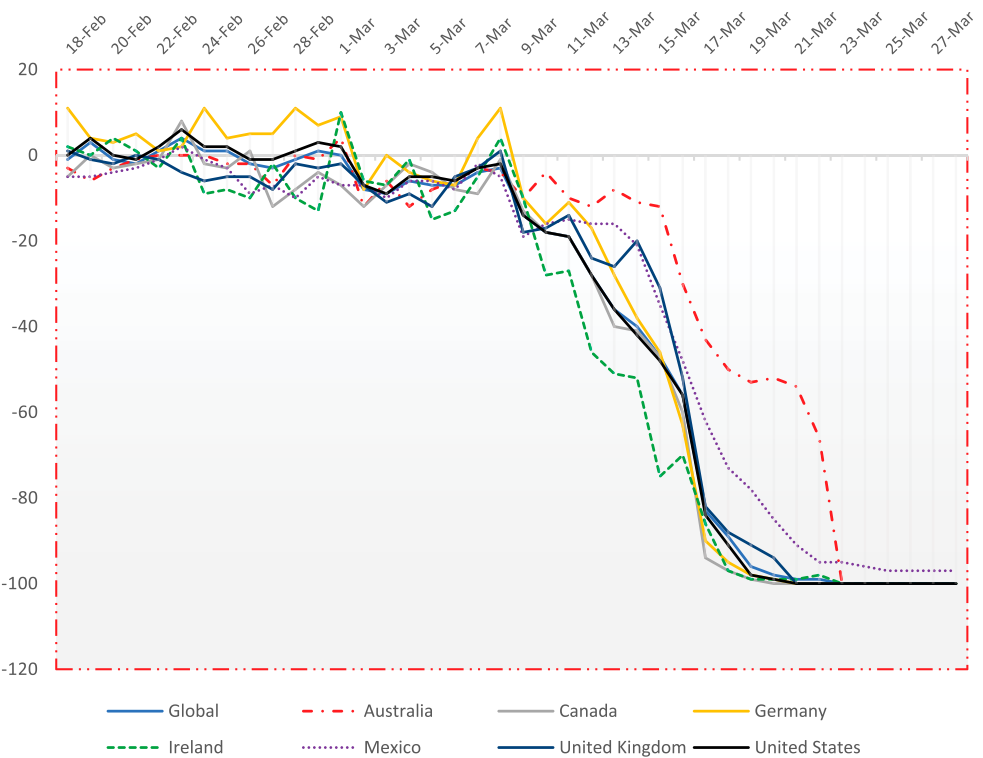
\includegraphics[width=\textwidth]{images/hChip/state-of-global-restaurant-industry-2020.png}
	\caption{Số liệu khách đến nhà hàng tại các nơi trên thế giới~\cite{dube2021covid}}
	\label{fig:state-of-global-restaurant-industry-2020}
\end{figure}

Mặc dù các ứng dụng đặt đồ ăn trực tuyến đã tồn tại từ lâu từ trước khi đại dịch xảy ra, nhưng khi khách hàng không còn lựa chọn ra ngoài ăn, số lượng người dùng mới đăng ký tham gia những nền tàng này tăng đáng kể xuyên suốt thời gian này~\cite{hoang2021customer}.
Các khảo sát sau đó cũng cho thấy rằng 64\%~\cite{pham2020study} người Việt Nam dự định tiếp tục sử dụng các ứng dụng đặt đồ ăn trong tương lai.
Như vậy từ sau đại dịch, đã có sự gia tăng một cách nhanh chóng trong thói quen đặt đồ ăn trực tuyến và mua hàng online của người dùng.
Khảo sát cũng cho thấy người dùng đặt ưu tiên về độ sạch sẽ của nhà hàng lên cao ngoài chất lượng món ăn khi họ đi ăn~\cite{hoang2021customer}.
Từ tất cả những điều trên, các quán ăn, nhà hàng mới chớm nở trong những năm trở lại đây đều gặp phải những trở ngại, thách thức nếu mong muốn mở rộng, phát triển và thu hút khách hàng tiềm năng đến với địa chỉ của họ.
Các quán ăn giờ đây cần phải chuyển dịch cơ cấu bán hàng của họ qua hình thức bán hàng trực tuyến~\cite{matsenko2021transformation}.
Điều này tức là mở rộng độ phủ của họ, tham gia vào các nền tảng bán hàng trực tuyến như Shopee Food, Grab Food, v.v..
Ngoài ra, việc thực khách giờ đây đặt ưu tiên sự sạch sẽ lên cao cũng tạo áp lực cho nhà hàng cần quản lý chặt chẽ nguồn cung của mình.
Đối với các quán ăn nhỏ lẻ, việc phát triển đồng thời hai phương thức bán hàng đó là bán hàng trực tuyến và bán hàng truyền thống rất tốn kém do chi phí đi kèm từ việc tham gia các nền tảng bán hàng trực tuyến đó là phí duy trì thành viên lên tới 25\% cho Shopee Food\footnote{https://merchant.shopeefood.vn/edu/article/phi-mo-gian-hang-va-chiet-khau-tren-shopeefood-la-bao-nhieu}.
Từ đây nhiều quán ăn chọn cách chuyển dịch cơ cấu sang chỉ buôn bán online nhằm giảm thiểu tối đa chi phí phát sinh cho việc thuê mặt bằng, chỗ ngồi cho khách hàng cũng như là chi phí cho các ứng dụng, hệ thống quản lý quán ăn.

Khóa luận này phát triển một giải pháp cho vấn đề nói trên.
Một hệ thống hỗ trợ quản lý nhà hàng, quán ăn cho các quán ăn tham gia dịch vụ.
Hệ thống cung cấp một ứng dụng cho phép các nhà hàng quản lý quán ăn của họ bao gồm quản lý nhân viên, thực đơn, thống kê doanh thu, hóa đơn theo các mốc thời gian cụ thể.
Ngoài ra nền tảng còn cung cấp giải pháp giúp các bên tham gia xây dựng nên một trang giới thiệu cho chính nhà hàng của họ đi kèm các dịch vụ như đặt bàn, hỗ trợ khách hàng, v.v..
Trong tương lai, hệ thống cũng hướng đến việc cho phép người dùng tạo lập tài khoản cho chính họ và cung cấp các tính năng giúp người dùng quản lý những thông tin như lịch sử ăn tại những nhà hàng, quán ăn họ đã đến và tìm kiếm các quán ăn dựa theo khẩu vị, địa điểm của người dùng.
Một khi người dùng đã có tài khoản trên nền tảng, các quán ăn, nhà hàng có thể biết được thông tin của người đến ăn nếu họ có trong hệ thống, từ đó đưa ra các chương trình khuyến mãi hợp lý cho bất kỳ thực khách quen nào tại chuỗi nhà hàng, quán ăn đó.

Phần còn lại của khóa luận được trình bày như sau.
Chương~\ref{chap1} trình bày giới thiệu về thiết kế tổng quan của hệ thống và các chức năng chính cũng như đi qua luồng nghiệp vụ của một số chức năng cụ thể.
Tiếp theo, Chương~\ref{chap2} mô tả chi tiết thêm về từng thành phần trong hệ thống, từ thiết kế của các cơ sở dữ liệu cho đến giao diện người dùng (màn hình) cho nhà hàng, quán ăn, khách hàng, v.v..
Chương~\ref{chap3} chia sẻ về quá trình cài đặt và triển khai hệ thống lên môi trường đám mây của Google, cài đặt các chứng chỉ web và tên miền, tích hợp CI/CD cho dự án giúp tự động hóa quá trình cài đặt và bảo mật.
Cuối cùng Chương~\ref{chap4} thực hiện đánh giá hệ thống sau khi đã triển khai, hiệu quả hoạt động và các vấn đề gặp phải trong quá trình chạy thực nghiệm.
Chương~\ref{chap4} cũng sẽ nói về một vài luồng người dùng khi thực hiện các chức năng cụ thể trong hệ thống bằng biểu đồ luồng tuần tự
\chapter{Giới thiệu hệ thống}\label{chap1}
Trước khi đi sâu vào thiết kế kiến trúc của hệ thống quản lý quán ăn và các dịch vụ liên quan, chương này sẽ trình bày một số kiến thức cơ bản, quan trọng liên quan đến đề tài, các khái niệm, công nghệ sử dụng cho dự án.
Sau khi đã có một cái nhìn tổng quan, Mục \autoref{sec:main-functions} giới thiệu những nhiệm vụ chính của hệ thống theo thiết kế ban đầu và mối liên hệ giữa từng dịch vụ trong hệ thống đối với từng chức năng.

\section{Kiến trúc hệ thống}
Nền tảng hạ tầng của hệ thống được thiết kế giúp hướng đến tính ổn định cao và phát triển cho sau này.
Khi hệ thống đạt một số lượng người dùng nhất định, và có thể những người dùng này trải dài khắp nơi thay vì tập trung chủ yếu tại một địa điểm cố định.
Khi đó, việc duy trì một máy chủ vật lý sẽ không còn là lựa chọn tối ưu do sự tốn kém về nhân lực cũng như chi phí phát sinh trong việc bảo trì và nâng cấp cho máy chủ.
Từ đó mô hình kiến trúc của dự án hướng tới triển khai trên môi trường đám mây, tức sử dụng máy chủ của các nhà cung cấp dịch vụ đám mây rải rác ở khắp nơi trên thế giới.
Điều này sẽ giúp giảm đáng kể thời gian cấu hình máy chủ vật lý của hệ thống cũng như thời gian cần phải bỏ ra giúp duy trì và bảo dưỡng do các tác nhân bên ngoài gây nên.

Hình \ref{fig:overall-architecture} dưới đây mô tả kiến trúc tổng quan của nền tảng quản lý quán ăn triển khai trên môi trường đám mây.

\begin{figure}[h]
	\centering
	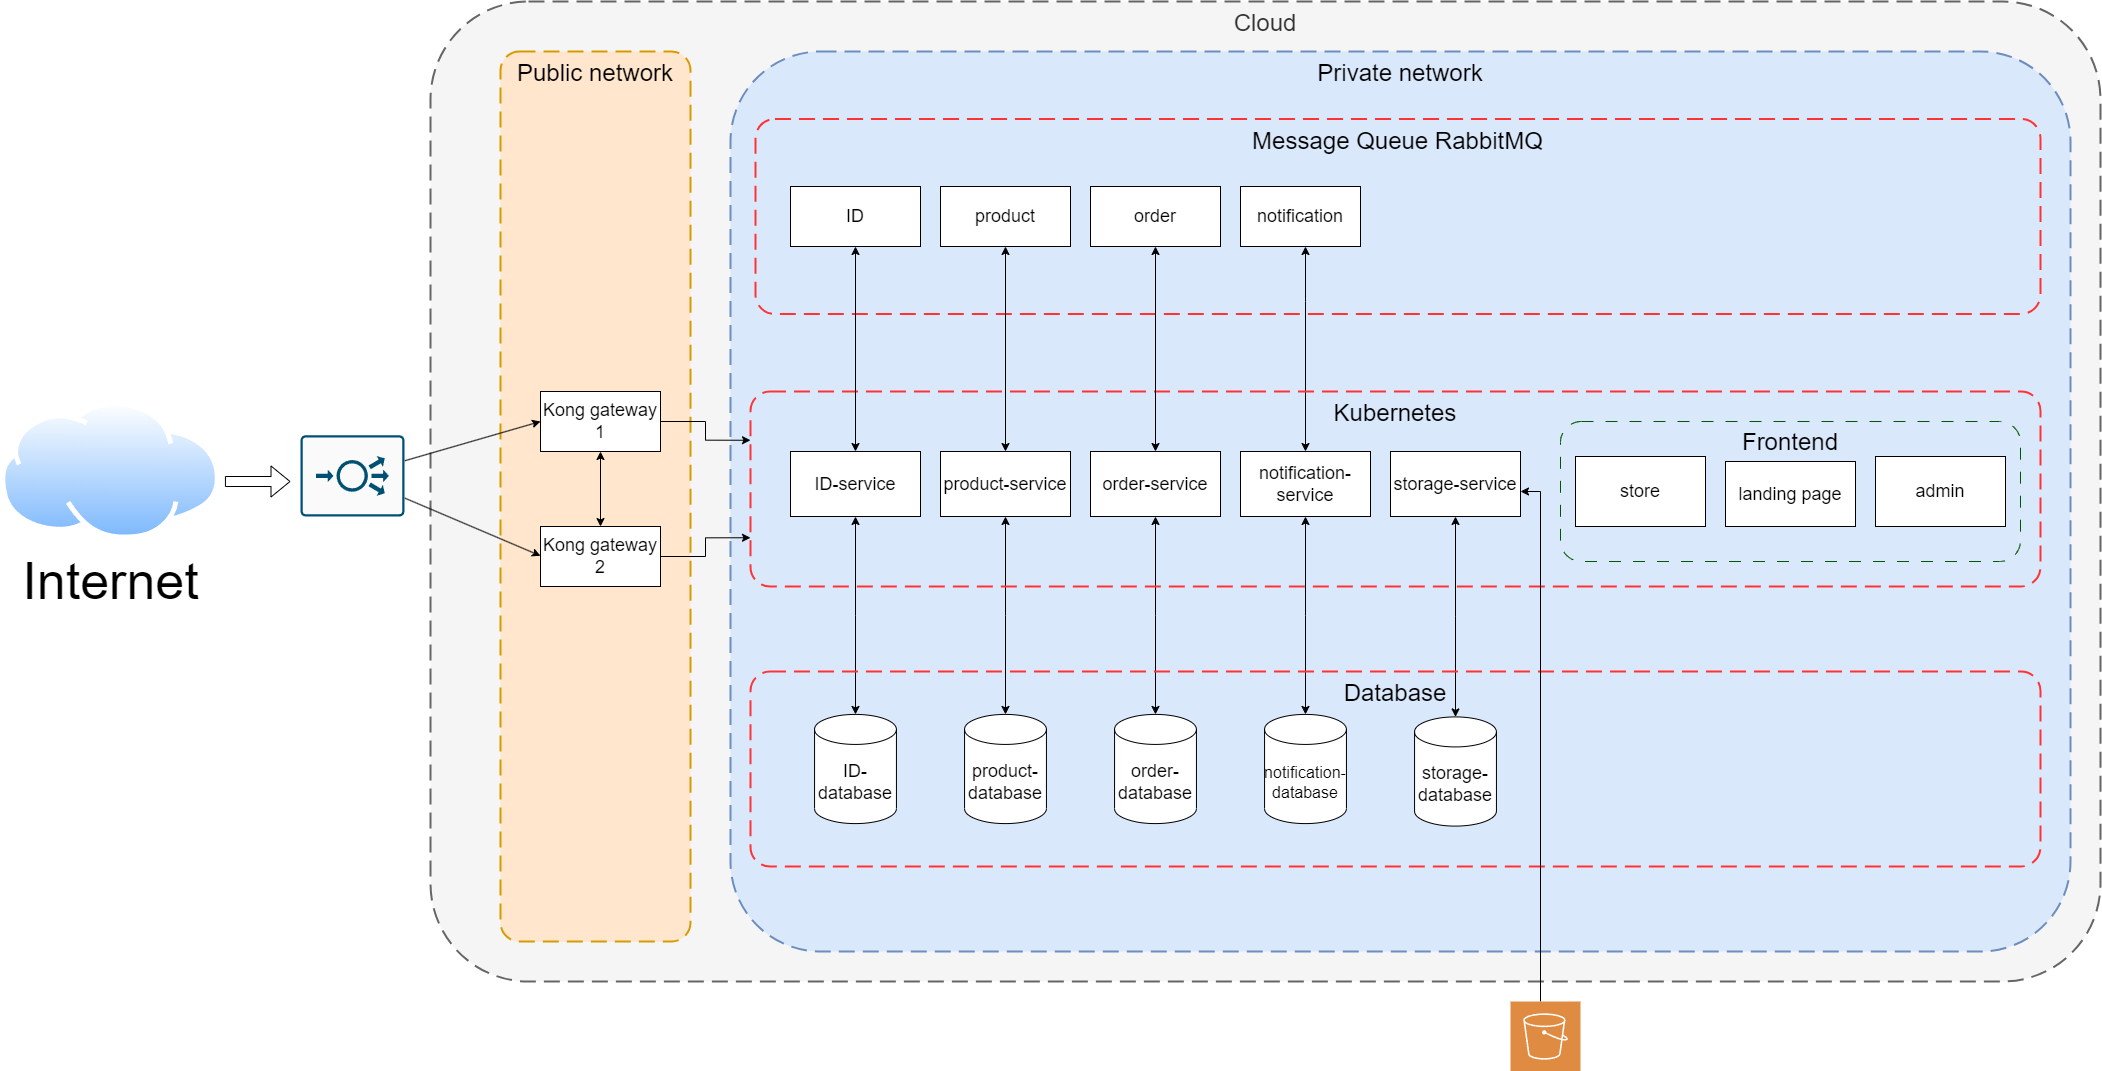
\includegraphics[width=1.1\textwidth]{images/hChip/overall-architecture.png}
	\caption{Hình vẽ mô tả kiến trúc tổng quan của hệ thống quản lý quán ăn}
	\label{fig:overall-architecture}
\end{figure}

Luồng dữ liệu đi vào hệ thống bắt nguồn từ ngoài Internet, nơi tất cả các yêu cầu của người dùng đi qua một GLSB (Global Server Load Balancers).
Ở đây GSLB của hệ thống được triển khai trên Cloudflare giúp phân phối người dùng ở bất cứ nơi nào trên thế giới đến máy chủ khỏe mạnh gần nhất đối với họ.
Điều này sẽ giúp tối ưu hóa thời gian tải trang, giảm thiểu độ trễ, và đảm bảo trải nghiệm truy cập website của người dùng nhanh chóng, mượt mà nhất.

Ngoài ra Cloudflare còn đóng vai trò như một hệ thống phân giải tên miền (DNS).
Khi người dùng truy cập vào trang của hệ thống lần đầu tiên trên trình duyệt web, trình duyệt sẽ gửi truy vấn tới máy chủ DNS cục bộ (resolver), thông thường sẽ là máy chủ của nhà mạng.
Máy chủ DNS cục bộ sẽ kiểm tra liệu tên miền đang được yêu cầu có địa chỉ IP tương ứng không, nếu không tìm thấy máy chủ DNS của nhà mạng sẽ thực hiện một lời gọi khác tới máy chủ DNS tại các cấp cao hơn.
Ở đây cấp độ ngay trên máy chủ cục bộ của nhà mạng sẽ là các máy chủ DNS nơi máy chủ được triển khai như Cloudflare hoặc Google Cloud.
Lời gọi sẽ được chuyển đến DNS của nhà cung cấp mạng của người dùng và sau đó là đến Cloudflare DNS.
Cloudflare sẽ nhận lời gọi của người dùng với tên miền của hệ thống đã được đăng ký trên Namecheap\footnote{https://www.namecheap.com/} và người dùng đến địa chỉ IP (Internet Protocol) của máy chủ phù hợp nhất với người gọi.

Bên trong mỗi máy chủ được triển khai trên Google Cloud sẽ có hai lớp mạng là mạng công cộng được phơi ra ngoài Internet và lớp mạng nội bộ nơi triển khai các thành phần chức năng chính.
Tại lớp mạng công cộng triển khai hai cổng API (API Gateway) phụ trợ cho nhau.
Ngoài những lợi ích chính của một cổng API đó là giúp thống nhất một điểm truy cập đến máy chủ thông qua API Gateway và cải thiện hiệu suất hệ thống nhờ cơ chế cache kết quả truy vấn API cũng như là giới hạn lưu lượng truy cập tránh quá tải, việc sử dụng song song hai cổng API cũng giúp phân phối lưu lượng truy cập giữa các cổng và giúp đảm bảo tính sẵn sàng cao cho hệ thống.

Các cổng API sau đó sẽ chuyển tiếp lời gọi từ ngoài Internet đến hệ thống mạng nội bộ của máy chủ, nơi sẽ triển khai các thành phần chính của mô hình quản lý quán ăn.
Hệ thống ở đây được chia thành ba lớp chính bao gồm lớp hàng đợi tin nhắn sử dụng RabbitMQ, lớp K8s bao gồm các dịch vụ phụ trách xử lý lời gọi của người dùng, và cuối cùng là lớp cơ sở dữ liệu lưu trữ các thông tin quan trọng như dữ liệu của người dùng, nhà hàng, quán ăn, v.v..
Hệ thống được thiết kế theo hướng kiến trúc vi dịch vụ (microservice) tức từng thành phần, chức năng chính của hệ thống sẽ được triển khai và hoạt động trên các môi trường độc lập với nhau giúp hệ thống chịu lỗi tốt hơn, bảo trì dễ dàng, và tiện lợi trong việc nâng cấp, mở rộng sau này.
Mỗi vi dịch vụ microservice có trách nhiệm thực hiện một chức năng cụ thể, ví dụ như dịch vụ thông báo sẽ hoạt động với mục đích duy nhất là nhận thông tin được đẩy đến từ một hoặc nhiều dịch vụ cụ thể và phân phối nó đến với các dịch vụ đã đăng ký nhận thông báo từ các dịch vụ đó.
Việc chia nhỏ hệ thống thành các dịch vụ độc lập mang lại nhiều lợi ích như giúp dễ dàng triển khai và bảo trì cho hệ thống, tăng tính sẵn sàng cũng như là khả năng chịu lỗi, giúp tự động mở rộng hệ thống.
Về mặt phát triển hệ thống, bởi vì mỗi vi dịch vụ đều hoàn toàn độc lập với nhau nên các đội ngũ phát triển của từng chức năng có thể chọn bộ công nghệ phù hợp nhất với nhu cầu và khả năng của đội.

Nền tảng quản lý quán ăn trên hình \ref{fig:overall-architecture} được triển khai nền tảng Kubernetes (K8s) và Google Cloud Platform (GCP) mang đến nhiều lợi ích cho việc vận hành và quản lý ứng dụng.
K8s là một nền tảng mã nguồn mở giúp tự động hóa việc triển khai, quản lý và mở rộng các ứng dụng đóng gói\footnote{https://kubernetes.io/docs/concepts/overview/}.
Sử dụng K8s cho hệ thống vi dịch vụ (microservice) giúp giảm tải đáng kể công sức triển khai từng dịch vụ độc lập một cũng như mở rộng, quản lý các dịch vụ này do K8s có thể được cấu hình để tự động hóa các tác vụ thủ công như tạo và quản lý các Docker container, tự động phục hồi và xử lý lỗi.
Các ưu điểm công nghệ của K8s sẽ được đề cập rõ hơn trong Chương \textcolor{red}{Trích dẫn đến phần chi tiết triển khai hệ thống khi cấu hình K8s cho từng pod}
GCP cung cấp một nền tảng đám mây với gói chức năng đa dạng kèm theo các công cụ hỗ trợ tốt cho hệ thống với kiến trúc vi dịch vụ (microservice) giúp dễ dàng triển khai và vận hành.
Có thể kể đến nền tảng GKE giúp người dùng cấu hình K8s trên GCP một cách dễ dàng, Firebase giúp bảo mật hệ thống, xác thực người dùng truy cập vào hệ thống thông qua việc tạo lập và quản lý tài khoản cả người dùng.
GCP cũng hỗ trợ người sử dụng tránh được các vấn đề liên quan đến cấu hình cơ sở hạ tầng của hệ thống.
Với các tùy chọn đa dạng, người dùng có thể dựa theo nhu cầu thực tế của hệ thống tại từng thời điểm và chọn cấu hình phù hợp.

Tất cả thông tin của người dùng cũng như là nhà hàng, quán ăn tham gia vào nền tảng đều sẽ được lưu trong cơ sở dữ liệu của hệ thống. Các thông tin này có thể là về những lần đặt bàn, thực đơn của quán ăn, những lần gọi món của người dùng, thông tin người dùng, v.v., hoặc thông tin của hệ thống như các chỉ số sức khỏe, các bản ghi hoạt động, v.v.. Nền tảng quản lý quán ăn của khóa luận hiện tại sử dụng MongoDB\footnote{https://www.mongodb.com/}, một cơ sở dữ liệu dạng NoSQL. Chi tiết về cơ sở dữ liệu sẽ được nói rõ hơn trong Mục \autoref{sec:tehcnologies-used}.

\section{Các chức năng chính}\label{sec:main-functions}
Mô hình quản lý quán ăn được phát triển trong khóa luận này sẽ tập trung vào các chức năng chính giúp nhà hàng, quán ăn quản lý thực đơn, khách và bàn, v.v..
Từ các chức năng chính như quản lý thực đơn sẽ có các chức năng nhỏ hơn bổ trợ cho chức năng chính.
Ví dụ như đối với chức năng quản lý bàn, ngoài các chức năng chính như tạo bàn mới, xóa bàn, thay đổi trạng thái của bàn, v.v., các nhánh chức năng phụ còn bao gồm các chức năng như ghép bàn, gán bàn cho những người đặt bàn trước, v.v..
Điều này giúp cho 

Hình \textcolor{red}{Vẽ UML từ Copy of hChip trên Miro và chuyển vào đây} mô tả các chức năng chính của mô hình quản lý quán ăn.


\section{Luồng nghiệp vụ} \label{sec:handle-undef}
Pha xử lý hàm thiếu định nghĩa được bổ sung với hai nhiệm vụ chính đó là xử lý nguyên mẫu hàm cơ bản thiếu định nghĩa tìm được bởi trình biên dịch và xử lý nguyên mẫu hàm ảo thiếu định nghĩa mà trình biên dịch không thể phát hiện được. Ý tưởng chung để giải quyết hai nhiệm vụ vừa đề cập dựa trên việc tìm kiếm các ứng viên nguyên mẫu hàm tương thích trong mã nguồn kiểm thử theo các tiêu chí thích hợp, sau đó sinh thân hàm giả cho các ứng viên này. Mục \autoref{sec:handle-undef-first} mô tả cụ thể về phương pháp xử lý nhiệm vụ thứ nhất. Phương pháp xử lý nguyên mẫu hàm ảo được trình bày trong Mục \autoref{sec:handle-undef-second}.

% \subsection{Xử lý nguyên mẫu hàm cơ bản thiếu định nghĩa tìm bởi trình biên dịch} \label{sec:handle-undef-first}
Khóa luận đề xuất phương pháp sử dụng trình biên dịch để tìm kiếm các nguyên mẫu hàm cần sinh thân hàm giả trong mã nguồn kiểm thử. Thuật toán \autoref{alg:handle-ref} mô tả chi tiết quá trình tìm kiếm và xử lý các nguyên mẫu hàm cơ bản thiếu định nghĩa. Trước hết, thuật toán bắt đầu bằng việc thu thập danh sách các nguyên mẫu hàm cơ bản cần quan tâm trong tập các tệp mã nguồn $S$ và khởi tạo tập $T$ rỗng. Danh sách trả về bao gồm các xâu ký tự, mỗi xâu biểu thị một hàm bao gồm tên hàm và danh sách tham số của hàm đó (dòng~1-2). Tập $T$ là tập hợp các nguyên mẫu hàm trong mã nguồn kiểm thử được sinh thân hàm giả. Sau khi có danh sách, thuật toán xử lý từng xâu trong danh sách đầu vào (dòng~3-14). Cụ thể, với mỗi xâu, một AST $undef\_ast$ được xây dựng từ chữ ký hàm mà xâu biểu thị (dòng~4). Tiếp đó, tên của nguyên mẫu hàm được trích xuất từ AST vừa xây dựng (dòng~5) và tập các nguyên mẫu hàm ứng viên có cùng tên trong mã nguồn kiểm thử được thu thập và lưu vào danh sách $candidates$ (dòng~6). Danh sách tham số của nguyên mẫu hàm $undef$ và phạm vi định danh (scope qualifier) được trích xuất từ AST phục vụ cho quá trình lọc (dòng~7-8). Danh sách ứng viên được lọc bởi Thuật toán~\ref{alg:filter-undef} và thu được các ứng viên hợp lệ $qualified\_cans$ (dòng~9). Cuối cùng, từng ứng viên hợp lệ $qc$ được sinh thân hàm giả và thêm vào tập $T$ (dòng~11-12). Dữ liệu trong tập $T$ được lưu lại để xây dựng môi trường kiểm thử cho mã nguồn đang xét trong các lần sau mà không cần xử lý lại từ đầu.

\begin{algorithm}[ht]
    \small
    \caption{Thuật toán xử lý hàm thiếu định nghĩa}
    \label{alg:handle-ref}
    \SetKwComment{Comment}{/* }{ */} 
    \KwIn{~$S$ - collection of source code files}
    \KwOut{~$T$ - collection of handled undefined functions}
					
    $undefined\_functions \leftarrow $ Get necessary undefined functions in $S$\;
    $T \leftarrow \emptyset$\;
    \For {$undef : undefined\_functions$} {
        $undef\_ast\leftarrow$ Construct AST from the string $undef$\;
        $undef\_name \leftarrow$ Get the name of the function from string $undef\_ast$\;
        $candidates \leftarrow$ Find all function prototypes having the same name with $undef\_name$ in source code\;
        $undef\_params \leftarrow$ Extract a list of parameters from $undef\_ast$\;
        $undef\_scope\leftarrow$ Extract function scope qualifier from $undef\_ast$\;
        $qualified\_cans\leftarrow$ \textbf{call} Algorithm \autoref{alg:filter-undef} $(undef\_params, undef\_scope, candidates)$\;
        \For {$qc : qualified\_cans$} {
            $t \leftarrow $ Generate simple function body for $qc$\;
            $T \leftarrow T \cup {t}$
        }
    }

    \Return $T$
\end{algorithm}

% \subsubsection*{Thu thập danh sách nguyên mẫu hàm cơ bản thiếu định nghĩa}\label{sec:find-undef}
Ý tưởng sử dụng các công cụ tiện ích của trình biên dịch để tìm nguyên mẫu hàm cần quan tâm xuất phát từ lợi thế trình biên dịch biết hàm nào sẽ được sử dụng trong các tệp đối tượng như đã trình bày ở Mục \autoref{sec:kno-undefine}. Đoạn mã \autoref{cod:command-undef} mô tả cách dùng các công cụ tiện ích có trong trình biên dịch để tìm các nguyên mẫu hàm thiếu định nghĩa. Đầu tiên, phương pháp đề xuất sử dụng công cụ \textit{g++} với cờ \textit{-c} để biên dịch các tệp mã nguồn thành tệp đối tượng (object file) có đuôi \textit{.o} (dòng 1). Sau đó, các tệp đối tượng này sẽ được liên kết bởi công cụ liên kết \textit{ld} và cờ \textit{-r} thành một tệp đối tượng tổng hợp \textit{temp.o} (dòng 2). Lí do phương pháp đề xuất sử dụng công cụ liên kết \textit{ld} thay vì \textit{g++} là bởi \textit{g++} yêu cầu người dùng phải hoàn thiện tất cả các nguyên mẫu hàm bị thiếu định nghĩa trước khi liên kết thành tệp tổng hợp. Cuối cùng, tệp đối tượng tổng hợp được phân tích bởi công cụ phân tích ký hiệu \textit{nm}\footnote{https://sourceware.org/binutils/docs/binutils/nm.html} với các cờ \textit{-u} - trích xuất các hàm thiếu định nghĩa, \textit{-C} - chuyển ký hiệu máy thành ngôn ngữ lập trình C++ (dòng 3). Đầu ra của công cụ \textit{nm} sẽ được ghi vào tệp \textit{list.txt}.\\

\begin{lstlisting}[language=C++, caption={Các câu lệnh tìm nguyên mẫu hàm thiếu định nghĩa cần quan tâm sử dụng trình biên dịch.}, label={cod:command-undef},  captionpos=b]
g++ -c *.cpp
ld -r *.o -o temp.o
nm temp.o -u -C > list.txt
\end{lstlisting}

\begin{figure}[t]
    \begin{minipage}[t]{0.49\linewidth}
    \begin{lstlisting}[language=C++, caption={Mã nguồn tệp a.cpp.}, label={cod:undef-cpp}, captionpos=b]
// a.cpp
#include "a.hpp"
#include "b.hpp"
    
int foo(A *a, int x) {
    int ret = a->bar(true);
    int max = maxT<int>(x, ret);
    max += a->echo();
    const int *p = &(a->x);
    ret -= func(p, max);
    return ret;
}

void gamma(A *a, int x) {
    double max = maxT<double>(x, a->x);
    a->x = max;
}
int unused(int x);
    \end{lstlisting}
    \end{minipage}
    \begin{minipage}[t]{0.49\linewidth}
    \begin{lstlisting}[language=C++, caption={Mã nguồn tệp a.hpp, b.hpp và c.hpp.}, label={cod:undef-hpp}, captionpos=b]
// a.hpp
#include "c.hpp"
class A {
public: 
    int x;
    A(int _x) { x = _x; }
    int bar(bool b);
    double echo() {
        return x + delta(&x);
    }
};
int bar(bool b);
// b.hpp
template <typename T> T max(T a);
int func(int *a, int b);
int func(const int* a, int b);
    
// c.hpp
double delta(int* const x);  
    \end{lstlisting}
\end{minipage}
\end{figure}

Các Đoạn mã \autoref{cod:undef-cpp}, \autoref{cod:undef-hpp} minh họa cách áp dụng phương pháp đề xuất trên tập đơn vị kiểm thử cần xử lý các nguyên mẫu hàm cơ bản thiếu định nghĩa với bốn tệp mã nguồn. Kiểm thử viên muốn kiểm thử tự động cho hai hàm có logic đầy đủ \tcode{foo} và \tcode{gamma}. Hai hàm này chứa mã nguồn đầy đủ. Hai đoạn mã chứa một số nguyên mẫu hàm đó là \tcode{unused}, \tcode{bar}, \tcode{delta} và ba hàm trong tệp \tcode{b.hpp}. Hàm \tcode{foo} trong Đoạn mã \autoref{cod:undef-cpp} nhận đầu vào là một biến con trỏ đến đối tượng của lớp \tcode{A} và một biến kiểu nguyên \tcode{x}. Logic mã nguồn của \tcode{foo} gọi tới hai phương thức của biến \tcode{a} đó là \tcode{bar} và \tcode{echo}. Ngoài ra, hàm \tcode{foo} còn gọi tới nguyên mẫu hàm template \tcode{maxT} với kiểu khởi tạo \tcode{int} và hàm \tcode{func(const int* a, int b)} thuộc tệp \tcode{b.hpp}. Hàm \tcode{gamma} cũng có các đầu vào tương tự nhưng gọi nguyên mẫu hàm \tcode{maxT} nhưng sử dụng tham số kiểu \tcode{double} thay vì \tcode{int} như hàm \tcode{foo}.
\vspace{5mm}
\begin{figure}[h]
	\begin{lstlisting}[language=C++, caption={Danh sách các nguyên mẫu hàm thiếu định nghĩa tìm bởi trình biên dịch.}, label={cod:result-undef}, captionpos=b]
func(int const*, int)
double maxT<double>(double, double)        
int maxT<int>(int, int)     
delta(int*)
A::bar(bool)         
	\end{lstlisting}
\end{figure}

Đoạn mã \autoref{cod:result-undef} minh họa danh sách các nguyên mẫu hàm cần quan tâm trong tệp các đơn vị kiểm thử \textit{a.cpp}, \textit{a.hpp}, \textit{b.hpp} và \textit{c.hpp} khi áp dụng phương pháp đề xuất. Dòng đầu tiên cho biết nguyên mẫu hàm \tcode{func(int const*, int)} cần được xử lý, tương đương với hàm \tcode{func(const int* a, int b)} trong mã nguồn \textit{b.hpp} (dòng 16 trong Đoạn~mã~\autoref{cod:undef-hpp}). Dòng 2 và 3 biểu thị cú pháp của hàm template. Đối với trình biên dịch, các lời gọi hàm template với các kiểu đối số khác nhau sẽ tạo ra các chữ ký hàm khác nhau. Do hàm \tcode{foo} và \tcode{gamma} gọi hàm \tcode{maxT} với hai đối số kiểu khác nhau nên danh sách các nguyên mẫu hàm thiếu định nghĩa chứa chữ ký hàm cho cả hai kiểu này. Tiếp theo, nguyên mẫu hàm ở dòng 4 tương ứng hàm \tcode{delta(int* const x)} trong tệp c.hpp. Tham số hiển thị ở tệp mã nguồn và trên danh sách khác nhau là bởi trình biên dịch chỉ quan tâm tới kiểu của tham số và loại bỏ lớp lưu trữ (storage class) ngoài cùng của tham số đó. Tham số \tcode{x} của hàm \tcode{delta} có kiểu là \tcode{int* const} tức con trỏ hằng trỏ tới một biến kiểu nguyên. Trình biên dịch chuyển kiểu của tham số trên thành \tcode{int*}. Trong trường hợp của hai hàm \tcode{func}, tham số đầu của hai hàm khác nhau là bởi tham số \tcode{const int* a} được trình biên dịch chuyển thành kiểu \tcode{const int*} do từ khoá \tcode{const} là lớp lưu trữ của biến được tham số trỏ tới. Cuối cùng nguyên mẫu hàm \tcode{A::bar(bool)} tương ứng với nguyên mẫu hàm \tcode{int bar(bool b)} trong lớp \tcode{A} (dòng 7 trong Đoạn mã \autoref{cod:undef-hpp}).

% \subsubsection*{Lọc tìm ứng viên hợp lệ}
Như đã mô tả trong ví dụ minh hoạ ở Đoạn mã \autoref{cod:result-undef}, mỗi nguyên mẫu hàm trong danh sách trả về bởi trình biên dịch sẽ tương ứng với một số nguyên mẫu hàm cơ bản trong mã nguồn gốc. Để ánh xạ từng nguyên mẫu hàm cần quan tâm tới đúng nguyên mẫu hàm cơ bản trong đơn vị kiểm thử, phương pháp đề xuất sử dụng ba tiêu chí để đánh giá độ phù hợp của từng ứng viên. Tiêu chí đầu tiên đó là hàm ứng viên chưa được ánh xạ bởi bất kỳ nguyên mẫu hàm nào trên danh sách. Tiêu chí thứ hai đó là số lượng tham số và phạm vi định danh của hai hàm phải giống nhau. Tiêu chí này giúp giảm số lượng các ứng viên có cùng tên cần xét. Cuối cùng, ứng viên hợp lệ nếu từng tham số đã chuẩn hoá của ứng viên có cùng kiểu với tham số tương ứng của nguyên mẫu hàm.
\begin{algorithm}
    \small
    \caption{Thuật toán lọc tìm ứng viên hợp lệ}
    \label{alg:filter-undef}
    \SetKwComment{Comment}{/* }{ */} 
    \KwIn{~$undef\_params$ - list of parameters extracted from the string $undef$ \\
    \hskip 1.1cm $undef\_scope$ - the scope qualifier of $undef$\\
    \hskip 1.1cm  $candidates$ - list of function prototypes having the same name
    }
    \KwOut{~$qualified\_cans$ - list of qualified function prototypes}
					
    $qualified\_cans \leftarrow$ Initial empty list\;
    \For {$candidate : candidates$} {
        \uIf {$candidate$ \textbf{is} \textit{handled}} {
            \textbf{continue}
        }
        \Else {
            $can\_params \leftarrow$ Extract a list of parameters of function $candidate$\;
            $can\_scope\leftarrow$ Get the scope qualifier of $candidate$\;
            \uIf {$can\_params.length \neq undef\_params.length$ \textbf{or} $can\_scope \neq undef\_scope$} {
                \textbf{continue}
            }
            \Else {
                $same\_params \leftarrow$ \textbf{True}\;
                $iter\leftarrow$ 1 \Comment*[r]{Assume the list starts at index 1}
                \While{$iter \leq can\_params.length$} {
                    $can\_param\_iter\leftarrow$ Normalize the $iter^{th}$ param of $can\_params$\;
                    $undef\_param\leftarrow$ Get the $iter^{th}$ param of $under\_params$ \;
                    \uIf{$can\_param\_iter$ \textbf{has the same type with} $under\_params$} {
                        $iter++$
                    }
                    \Else {
                        $same\_params\leftarrow$ \textbf{False}\;
                        \textbf{break}
                    }
                }

                \If{$same\_params\leftarrow$ \textbf{True}} {
                    Set $candidate$ state to $handled$\;
                    Push $candidate$ into $qualified\_cans$\;
                }
            }
        }
    }
    \KwRet{$qualified\_cans$}
\end{algorithm}

Thuật toán \autoref{alg:filter-undef} mô tả chi tiết cách áp dụng ba tiêu chí để lọc ra các ứng viên hợp lệ. Đầu vào của thuật toán gồm danh sách tham số trích xuất từ nguyên mẫu hàm cần tìm và danh sách nguyên mẫu hàm ứng viên trong mã nguồn kiểm thử. Mỗi ứng viên sẽ được xét duyệt lần lượt trên ba tiêu chí (dòng 3-28). Nếu ứng viên $candidate$ đã được ánh xạ (hay có trạng thái $handled$), ứng viên sẽ được bỏ qua (dòng 3-4). Ngược lại, danh sách tham số của ứng viên $candidate$ được trích xuất để sử dụng cho hai tiêu chí còn lại (dòng~6). Nếu số lượng tham số hoặc phạm vi định danh của ứng viên khác nguyên mẫu hàm đầu vào thì ứng viên này sẽ được bỏ qua (dòng~8-9). Để áp dụng tiêu chí thứ ba một cách hiệu quả, phương pháp đề xuất xét duyệt lần lượt từng tham số và dừng lại khi gặp tham số đầu tiên không hợp lệ. Trước hết, thuật toán khởi tạo biến $same\_params$ dùng để đánh dấu tất cả tham số đều hợp lệ và gán biến $iter$ bằng vị trí đầu tiên trong danh sách tham số (dòng~11-12). Tiếp đó, quá trình lặp đánh giá từng tham số diễn ra cho đến hết danh sách tham số hoặc gặp tham số không hợp lệ (dòng~13-22). Tham số thứ $iter$ của ứng viên và hàm đầu vào được lấy ra (dòng~13-14). Do tham số của hàm đầu vào đã được chuẩn hoá theo tiêu chuẩn của C++\footnote{https://www.open-std.org/jtc1/sc22/wg21/docs/standards}\footnote{https://en.cppreference.com/w/cpp/language/function} nên tham số của ứng viên cũng sẽ được đưa về theo các tiêu chuẩn này. Nếu hai tham số đang xét có cùng kiểu thì thuật toán sẽ chuyển sang tham số tiếp theo (dòng 16-17). Ngược lại, quá trình lặp sẽ kết thúc và thuật toán đánh dấu tính hợp lệ là $False$ (dòng 19-20). Sau quá trình đánh giá, nếu tất cả tham số của ứng viên đều hợp lệ, thuật toán chuyển trạng thái của ứng viên thành đã được ánh xạ và thêm vào danh sách ứng viên hợp lệ.
\chapter{Thiết kế hệ thống}\label{chap2}
\section{Kiến trúc hệ thống}
% \subsection{Cây cú pháp trừu tượng và đồ thị dòng điều khiển} \label{sec:kno-ast-and-cfg}
Nền tảng hạ tầng của hệ thống được thiết kế giúp hướng đến tính ổn định cao và phát triển cho sau này.
Khi hệ thống đạt một số lượng người dùng nhất định, và có thể những người dùng này trải dài khắp nơi thay vì tập trung chủ yếu tại một địa điểm cố định.
Khi đó, việc duy trì một máy chủ vật lý sẽ không còn là lựa chọn tối ưu do sự tốn kém về nhân lực cũng như chi phí phát sinh trong việc bảo trì và nâng cấp cho máy chủ.
Từ đó mô hình kiến trúc của dự án hướng tới triển khai trên môi trường đám mây, tức sử dụng máy chủ của các nhà cung cấp dịch vụ đám mây rải rác ở khắp nơi trên thế giới.
Điều này sẽ giúp giảm đáng kể thời gian cấu hình máy chủ vật lý của hệ thống cũng như thời gian cần phải bỏ ra giúp duy trì và bảo dưỡng do các tác nhân bên ngoài gây nên.

Hình \ref{fig:overall-architecture} dưới đây mô tả kiến trúc tổng quan của nền tảng quản lý quán ăn triển khai trên môi trường đám mây.

\begin{figure}[h]
	\centering
	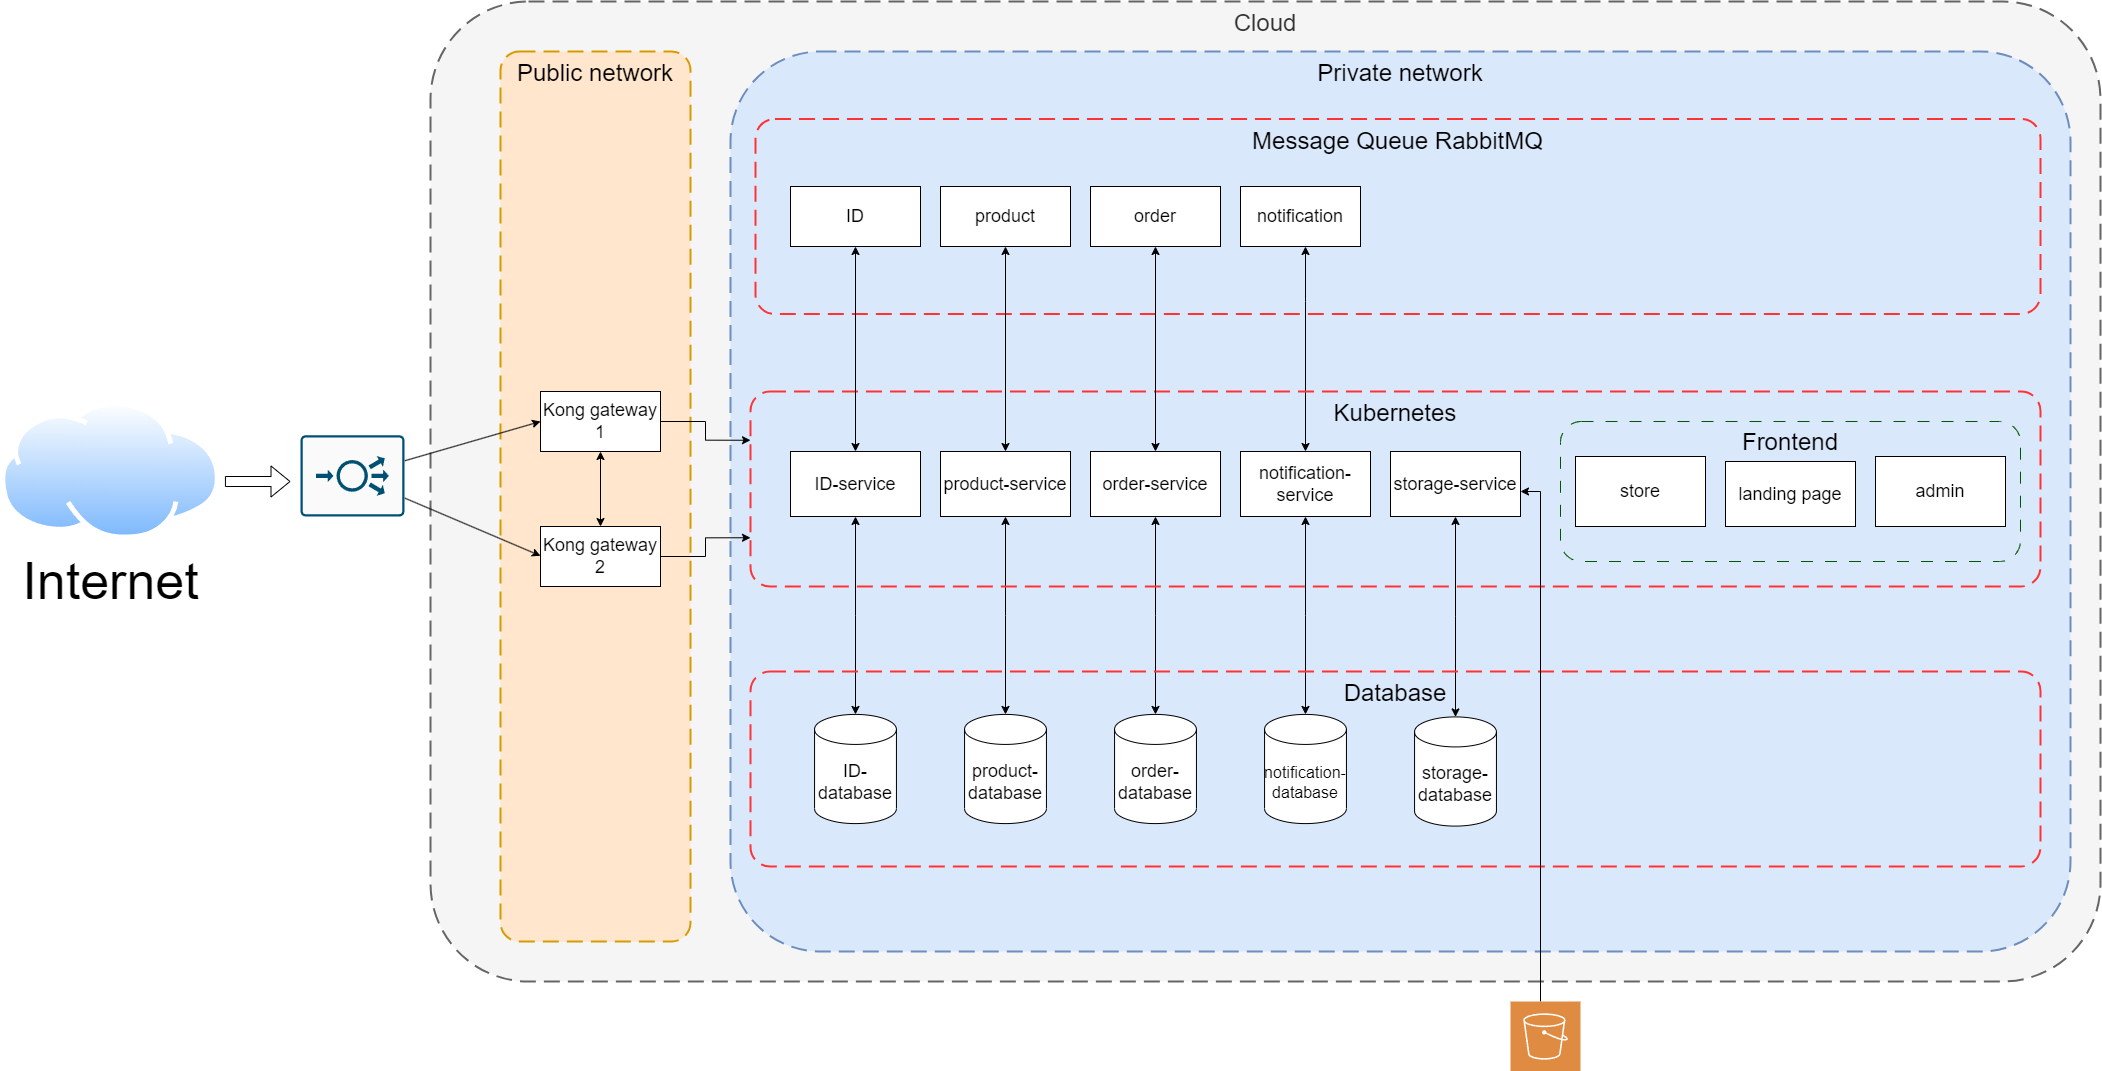
\includegraphics[width=1.1\textwidth]{images/hChip/overall-architecture.png}
	\caption{Hình vẽ mô tả kiến trúc tổng quan của hệ thống quản lý quán ăn}
	\label{fig:overall-architecture}
\end{figure}

Luồng dữ liệu đi vào hệ thống bắt nguồn từ ngoài Internet, nơi tất cả các yêu cầu của người dùng đi qua một GLSB (Global Server Load Balancers).
Ở đây GSLB của hệ thống được triển khai trên Cloudflare giúp phân phối người dùng ở bất cứ nơi nào trên thế giới đến máy chủ khỏe mạnh gần nhất đối với họ.
Điều này sẽ giúp tối ưu hóa thời gian tải trang, giảm thiểu độ trễ, và đảm bảo trải nghiệm truy cập website của người dùng nhanh chóng, mượt mà nhất.

Ngoài ra Cloudflare còn đóng vai trò như một hệ thống phân giải tên miền (DNS).
Khi người dùng truy cập vào trang của hệ thống lần đầu tiên trên trình duyệt web, trình duyệt sẽ gửi truy vấn tới máy chủ DNS cục bộ (resolver), thông thường sẽ là máy chủ của nhà mạng.
Máy chủ DNS cục bộ sẽ kiểm tra liệu tên miền đang được yêu cầu có địa chỉ IP tương ứng không, nếu không tìm thấy máy chủ DNS của nhà mạng sẽ thực hiện một lời gọi khác tới máy chủ DNS tại các cấp cao hơn.
Ở đây cấp độ ngay trên máy chủ cục bộ của nhà mạng sẽ là các máy chủ DNS nơi máy chủ được triển khai như Cloudflare hoặc Google Cloud.
Lời gọi sẽ được chuyển đến DNS của nhà cung cấp mạng của người dùng và sau đó là đến Cloudflare DNS.
Cloudflare sẽ nhận lời gọi của người dùng với tên miền của hệ thống đã được đăng ký trên Namecheap\footnote{https://www.namecheap.com/} và người dùng đến địa chỉ IP (Internet Protocol) của máy chủ phù hợp nhất với người gọi.

Bên trong mỗi máy chủ được triển khai trên Google Cloud sẽ có hai lớp mạng là mạng công cộng được phơi ra ngoài Internet và lớp mạng nội bộ nơi triển khai các thành phần chức năng chính.
Tại lớp mạng công cộng triển khai hai cổng API (API Gateway) phụ trợ cho nhau.
Ngoài những lợi ích chính của một cổng API đó là giúp thống nhất một điểm truy cập đến máy chủ thông qua API Gateway và cải thiện hiệu suất hệ thống nhờ cơ chế cache kết quả truy vấn API cũng như là giới hạn lưu lượng truy cập tránh quá tải, việc sử dụng song song hai cổng API cũng giúp phân phối lưu lượng truy cập giữa các cổng và giúp đảm bảo tính sẵn sàng cao cho hệ thống.

Các cổng API sau đó sẽ chuyển tiếp lời gọi từ ngoài Internet đến hệ thống mạng nội bộ của máy chủ, nơi sẽ triển khai các thành phần chính của mô hình quản lý quán ăn.
Hệ thống ở đây được chia thành ba lớp chính bao gồm lớp hàng đợi tin nhắn sử dụng RabbitMQ, lớp K8s bao gồm các dịch vụ phụ trách xử lý lời gọi của người dùng, và cuối cùng là lớp cơ sở dữ liệu lưu trữ các thông tin quan trọng như dữ liệu của người dùng, nhà hàng, quán ăn, v.v..
Hệ thống được thiết kế theo hướng kiến trúc vi dịch vụ (microservice) tức từng thành phần, chức năng chính của hệ thống sẽ được triển khai và hoạt động trên các môi trường độc lập với nhau giúp hệ thống chịu lỗi tốt hơn, bảo trì dễ dàng, và tiện lợi trong việc nâng cấp, mở rộng sau này.
Mỗi vi dịch vụ microservice có trách nhiệm thực hiện một chức năng cụ thể, ví dụ như dịch vụ thông báo sẽ hoạt động với mục đích duy nhất là nhận thông tin được đẩy đến từ một hoặc nhiều dịch vụ cụ thể và phân phối nó đến với các dịch vụ đã đăng ký nhận thông báo từ các dịch vụ đó.
Việc chia nhỏ hệ thống thành các dịch vụ độc lập mang lại nhiều lợi ích như giúp dễ dàng triển khai và bảo trì cho hệ thống, tăng tính sẵn sàng cũng như là khả năng chịu lỗi, giúp tự động mở rộng hệ thống.
Về mặt phát triển hệ thống, bởi vì mỗi vi dịch vụ đều hoàn toàn độc lập với nhau nên các đội ngũ phát triển của từng chức năng có thể chọn bộ công nghệ phù hợp nhất với nhu cầu và khả năng của đội.

Nền tảng quản lý quán ăn trên hình \ref{fig:overall-architecture} được triển khai nền tảng Kubernetes (K8s) và Google Cloud Platform (GCP) mang đến nhiều lợi ích cho việc vận hành và quản lý ứng dụng.
K8s là một nền tảng mã nguồn mở giúp tự động hóa việc triển khai, quản lý và mở rộng các ứng dụng đóng gói\footnote{https://kubernetes.io/docs/concepts/overview/}.
Sử dụng K8s cho hệ thống vi dịch vụ (microservice) giúp giảm tải đáng kể công sức triển khai từng dịch vụ độc lập một cũng như mở rộng, quản lý các dịch vụ này do K8s có thể được cấu hình để tự động hóa các tác vụ thủ công như tạo và quản lý các Docker container, tự động phục hồi và xử lý lỗi.
Các ưu điểm công nghệ của K8s sẽ được đề cập rõ hơn trong Chương \textcolor{red}{Trích dẫn đến phần chi tiết triển khai hệ thống khi cấu hình K8s cho từng pod}
GCP cung cấp một nền tảng đám mây với gói chức năng đa dạng kèm theo các công cụ hỗ trợ tốt cho hệ thống với kiến trúc vi dịch vụ (microservice) giúp dễ dàng triển khai và vận hành.
Có thể kể đến nền tảng GKE giúp người dùng cấu hình K8s trên GCP một cách dễ dàng, Firebase giúp bảo mật hệ thống, xác thực người dùng truy cập vào hệ thống thông qua việc tạo lập và quản lý tài khoản cả người dùng.
GCP cũng hỗ trợ người sử dụng tránh được các vấn đề liên quan đến cấu hình cơ sở hạ tầng của hệ thống.
Với các tùy chọn đa dạng, người dùng có thể dựa theo nhu cầu thực tế của hệ thống tại từng thời điểm và chọn cấu hình phù hợp.

Tất cả thông tin của người dùng cũng như là nhà hàng, quán ăn tham gia vào nền tảng đều sẽ được lưu trong cơ sở dữ liệu của hệ thống. Các thông tin này có thể là về những lần đặt bàn, thực đơn của quán ăn, những lần gọi món của người dùng, thông tin người dùng, v.v., hoặc thông tin của hệ thống như các chỉ số sức khỏe, các bản ghi hoạt động, v.v.. Nền tảng quản lý quán ăn của khóa luận hiện tại sử dụng MongoDB\footnote{https://www.mongodb.com/}, một cơ sở dữ liệu dạng NoSQL. Chi tiết về cơ sở dữ liệu sẽ được nói rõ hơn trong Mục \autoref{sec:tehcnologies-used}.

\section{Cấu trúc cơ sở dữ liệu} \label{sec:database-design}
Như đã đề cập ở Mục \autoref{sec:tongquan}, pha xây dựng môi trường kiểm thử thực hiện hai nhiệm vụ chính. Nhiệm vụ thứ nhất đó là thực hiện hai tác vụ tiền xử lý mã nguồn. Tác vụ đầu tiên là tác vụ thiết lập môi trường nhằm biên dịch mã nguồn và các ca kiểm thử về sau. Tác vụ này cài đặt các lệnh biên dịch, xác định và liên kết các thư viện mà mã nguồn sử dụng, thiết lập kiểu độ phủ mong muốn cho các đơn vị kiểm thử. Tác vụ thứ hai là tác vụ tạo môi trường tính toán độ phủ. Tác vụ này nhân bản mã nguồn kiểm thử và bổ sung các câu lệnh đánh dấu nhằm phục vụ quá trình xác định các câu lệnh, nhánh được viếng thăm và tính toán độ phủ trong pha sinh dữ liệu kiểm thử tự động. Nhiệm vụ còn lại của pha đó là phân tích mã nguồn kiểm thử và xây dựng đồ thị cấu trúc mã nguồn. Bước phân tích mã nguồn sử dụng công cụ phân tích mã nguồn CDT Parser\footnote{https://github.com/eclipse-cdt/cdt} để trích xuất AST của mã nguồn kiểm thử. Từ thông tin trên AST, phương pháp đề xuất xây dựng đồ thị cấu trúc mã nguồn với các thông tin được phân tích đến mức hàm.

% \subsection*{Đồ thị cấu trúc mã nguồn}
Đồ thị cấu trúc mã nguồn là một cấu trúc dữ liệu biểu diễn mối quan hệ và sự tương tác giữa các thành phần trong mã nguồn kiểm thử. Đồ thị này được biểu diễn bởi một đồ thị có hướng $G = (V, E)$, trong đó $V$ là tập các đỉnh tượng trưng cho các thành phần trong các đơn vị kiểm thử và $E$ là tập các cạnh có hướng nối giữa hai đỉnh tượng trưng cho mối quan hệ phát sinh giữa đỉnh đầu và đỉnh cuối. Mỗi đỉnh trong đồ thị biểu thị cho các đơn vị cơ bản như như tệp mã nguồn, lớp, biến, thư viện được sử dụng, các hàm, v.v. Để làm rõ thể hiện của các hàm thiếu định nghĩa trong đồ thị, khóa luận biểu thị hàm thành hai loại đỉnh hàm: đỉnh nguyên mẫu hàm và đỉnh định nghĩa hàm. Các hàm được khai báo đầy đủ biểu thị bởi đỉnh định nghĩa hàm. Mỗi cạnh trong mã nguồn thuộc một trong các cạnh được mô tả dưới đây.
\begin{itemize}
    \item Cạnh cha con: Thể hiện mối quan hệ cha - con (hay mối quan hệ chứa) giữa hai đơn vị cơ bản trong đơn vị kiểm thử. Ví dụ cho mối quan hệ này có thể kể đến như lớp chứa một số thuộc tính và phương thức, tương đương quan hệ lớp là cha của các thuộc tính và phương thức.
    \item Cạnh Include: Thể hiện mối quan hệ Include giữa hai tệp mã nguồn. Ví dụ cho quan hệ này là dòng lệnh \tcode{\#include} thường thấy trong các mã nguồn C/C++.
    \item Cạnh kế thừa: Thể hiện mối quan hệ kế thừa giữa lớp cha và lớp dẫn xuất. Hai đỉnh của cạnh là hai đỉnh lớp.
    \item Cạnh lời gọi hàm: Thể hiện tương tác giữa hai hàm trong mã nguồn kiểm thử. Hai đỉnh của cạnh là hai đỉnh hàm. Cạnh lời gọi hàm là thành phần quan trọng trong bước xác định các hàm cần tạo stub khi kiểm thử tự động cho một hầm bất kì.
    \item Cạnh định nghĩa: Thể hiện mối quan hệ định nghĩa giữa đỉnh nguyên mẫu hàm ảo và đỉnh định nghĩa hàm ảo. Quan hệ định nghĩa thể hiện nguyên mẫu hàm được trỏ tới tồn tại một khai báo định nghĩa.
\end{itemize}

Đồ thị cấu trúc mã nguồn được xây dựng bằng việc mở rộng từng đỉnh tệp với các cạnh cha con. Quá trình mở rộng đỉnh tệp cấu thành một cây cấu trúc tệp. Tiếp theo, dựa trên các cây cấu trúc tệp, đồ thị cấu trúc mã nguồn được hoàn thiện bằng cách phân tích AST kết hợp tìm kiếm để bổ sung các cạnh quan hệ còn lại. Cạnh định nghĩa là trường hợp đặc biệt được bổ sung sau vào đồ thị trong pha xử lý hàm thiếu định nghĩa.

% \subsection*{Ví dụ về đồ thị cấu trúc mã nguồn}
Hình \autoref{fig:dep-graph} minh hoạ đồ thị cấu trúc mã nguồn của hai tệp mã nguồn a.hpp và a.cpp trong các Đoạn mã \autoref{cod:dep-cpp}, \autoref{cod:dep-hpp}. Trong đó, các cạnh nét liền mũi tên đen thể hiện cạnh cha con giữa hai đỉnh và các kiểu cạnh còn lại được ký hiệu trên hình vẽ với thể hiện tương ứng. Cây cấu trúc mã nguồn của tệp \textit{a.cpp} gồm ba đỉnh hàm. Cây cấu trúc mã nguồn của tệp \textit{a.hpp} gồm hai đỉnh lớp, mỗi đỉnh lớp có quan hệ cha con với một số đỉnh như đỉnh thuộc tính, đỉnh nguyên mẫu hàm. Cạnh Include từ đỉnh tệp \textit{a.cpp} tới đỉnh \textit{a.hpp} tương đương dòng lệnh \tcode{\#include "a.hpp"} trong Đoạn mã \autoref{cod:dep-cpp}. Cạnh lời gọi hàm từ đỉnh định nghĩa hàm \tcode{double A::foo()} tới đỉnh định nghĩa hàm \tcode{int stub()} tương đương lời gọi hàm ở dòng 8 trong tệp \textit{a.cpp}. Đoạn mã ví dụ cho thấy nguyên mẫu hàm ảo \tcode{int func()} trong lớp A có tồn tại định nghĩa bởi hàm \tcode{int A::func()} nhưng đồ thị thiếu cạnh định nghĩa về quan hệ này do cạnh định nghĩa giữa hai đỉnh sẽ được bổ sung sau pha xử lý hàm thiếu định nghĩa.  

\begin{figure}[H]
	\begin{minipage}[t]{0.49\linewidth}
		\begin{lstlisting}[language=C++, caption={Mã nguồn tệp \textit{a.cpp} minh họa đồ thị cấu trúc mã nguồn.}, label={cod:dep-cpp}, captionpos=b]
// a.cpp
#include "a.hpp"
int A::func() {
	/* Function logic */
}
double foo() {
	/* Some logic */
	int ret = stub();
	/* Some logic */
}
int stub() {
	/* Function logic */
}
		\end{lstlisting}
	\end{minipage}
	\begin{minipage}[t]{0.49\linewidth}
		\begin{lstlisting}[language=C++, caption={Mã nguồn tệp \textit{a.hpp} minh họa đồ thị cấu trúc mã nguồn.}, label={cod:dep-hpp}, captionpos=b]
// a.hpp
class IA {
	public: 
	int bar();
};
class A : public IA {
	public:
	A() {}
	int x;
	virtual int beta();
	virtual int func();
	double foo();
}; 
		\end{lstlisting}
	\end{minipage}
			
	\vspace{1cm}
    \includesvg[width=\linewidth]{images/dep-graph}
    \caption{Ví dụ minh hoạ về đồ thị cấu trúc mã nguồn xây dựng trên mã nguồn tệp \textit{a.hpp} và \textit{a.cpp}.}
    \label{fig:dep-graph}
\end{figure}

\section{Giao diện người dùng}\label{sec:UI}
Về tổng quan, phương pháp đề xuất là sự kết hợp giữa phương pháp kiểm thử tượng trưng động~\cite{ConcolicTesting} và phương pháp sinh giả lập mã nguồn tự động~\cite{TUNG2022106821} với các cải tiến trong quá trình xử lý môi trường kiểm thử chứa hàm thiếu định nghĩa và quá trình thực thi tượng trưng lời gọi phương thức. Quá trình kiểm thử tự động bao gồm bốn pha được mô tả trong Hình~\autoref{fig:proposed-flow}. Các pha được in đậm trong hình vẽ thể hiện chúng được bổ sung hoặc cải tiến bởi phương pháp đề xuất.

\begin{figure}[h]
    \centering
    \includesvg[width=\linewidth]{images/proposed-flow}
    \caption{Tổng quan phương pháp đề xuất.}
    \label{fig:proposed-flow}
\end{figure}

Pha đầu tiên trong phương pháp đề xuất là pha xây dựng môi trường kiểm thử. Hai nhiệm vụ chính của pha đó là thực hiện các tác vụ tiền xử lý trên mã nguồn kiểm thử và phân tích mã nguồn để xây dựng đồ thị cấu trúc mã nguồn kiểm thử. Nội dung chi tiết của pha xây dựng môi trường kiểm thử được trình bày trong Mục~\autoref{sec:3-build-env}.

Pha tiếp theo trong phương pháp đề xuất là pha xử lý hàm thiếu nghĩa. Pha này được bổ sung so với phương pháp kiểm thử tự động truyền thống nhằm xử lý các vấn đề phát sinh bởi các hàm thiếu định nghĩa khi kiểm thử tự động cho các mã nguồn chưa hoàn chỉnh. Chi tiết về quá trình xử lý hàm thiếu định nghĩa được mô tả trong Mục~\autoref{sec:handle-undef}.

Sau pha xử lý hàm thiếu định nghĩa, quá trình kiểm thử tự động chuyển sang pha sinh dữ liệu kiểm thử tự động cho các đơn vị kiểm thử. Khóa luận sử dụng phương pháp sinh kế thừa từ phương pháp sinh dữ liệu kiểm thử tượng trưng động và phương pháp sinh giả lập mã nguồn AS4UT (mô tả ở Mục~\autoref{sec:autostub-Lam}). Trong pha sinh dữ liệu kiểm thử tự động, phương pháp đề xuất bổ sung bước sinh giả lập mã nguồn cho các hàm là phương thức của đối tượng nhằm tăng khả năng thực thi các câu lệnh, điều kiện có liên quan đến các đối tượng được sử dụng trong đơn vị kiểm thử. Nội dung chi tiết của pha sinh dữ liệu kiểm thử được trình bày ở Mục~\autoref{sec:autogen}. 

Cuối cùng, các dữ liệu độ phủ được thu thập ở pha sinh dữ liệu kiểm thử được phân tích và tạo thành báo cáo kiểm thử trong pha sinh báo cáo độ phủ mã nguồn. Khóa luận sử dụng công cụ tính độ phủ GNU Coverage - GCOV\footnote{https://gcc.gnu.org/onlinedocs/gcc/Gcov-Intro.html} và công cụ sinh báo cáo độ phủ LCOV để thực hiện nhiệm vụ của pha. Trong đó, GCOV là công cụ phân tích độ phủ tích hợp sẵn trong tập hợp các trình biên dịch GNU (GNU Compiler Collection - GCC), LCOV là một tiện ích mở rộng từ công cụ GCOV với nhiệm vụ sinh báo cáo độ phủ dạng ngôn ngữ siêu văn bản (Hypertext Markup Language - HTML) dựa trên các thông tin độ phủ của GCOV. GCOV và LCOV là hai công cụ có sẵn trong GCC và được sử dụng phổ biến trong các dự án~C/C++ \cite{hu2021software}. Quá trình thực thi ca kiểm thử ở pha trước sinh ra thông tin về số lần chạy qua một dòng, số lần chạy qua các nhánh điều kiện với từng trường hợp đúng, sai theo định dạng của GCOV. Thông tin này sau đó được LCOV tổng hợp, tính toán và đưa ra tệp báo cáo HTML.
\chapter{Triển khai hệ thống}\label{chap3}
Ở Chương~\nameref{chap2} khóa luận đã đề cập đến một số công nghệ được sử dụng trong quá trình thiết kế như Kubernetes, RabbitMQ, MongoDB, v.v.
Mỗi công nghệ được lựa chọn và sử dụng trong quá trình phát triển hệ thống đều đóng một vai trò quan trọng giúp đảm bảo luồng nghiệp vụ phía người dùng diễn ra một cách mượt mà và toàn vẹn.
Chương này sẽ đi chi tiết hơn vào diễn giải cách các công nghệ này tương tác, hoạt động với nhau, lợi ích của từng công nghệ cụ thể.
Tiếp sau đó, Mục~\nameref{sec:deploy-environment} sẽ trình bày cách triển khai hệ thống quản lý quán ăn lên môi trường đám mây của Google Cloud quá trình cài đặt HPA giúp hệ thống tự động mở rộng (autoscale) khi có lưu lượng truy cập lớn.
\section{Công nghệ sử dụng} \label{sec:tehcnologies-used}
\subsection{Kubernetes (K8s)}
Đối với mô hình quản lý quán ăn tập trung, việc đảm bảo khả năng chịu lỗi và tính sẵn sàng cao khi các quán ăn sử dụng hệ thống là điều thiết yếu.
Điều này đặc biệt đúng trong giờ cao điểm khi các nhà hàng, quán ăn đón một lượng lớn khách hàng đến quán.
Từ đó khóa luận này đưa ra phương án thiết kế hệ thống đi theo mô hình hệ thống phân tán (distributed system) với kiến trúc vi dịch vụ sử dụng K8s nhằm đạt được những yêu cầu đề ra và hơn thế nữa.

Khi sử dụng mô hình phân tán, hệ thống sẽ tránh được việc có một điểm lỗi duy nhất (single point of failure), khi một dịch vụ ngừng hoạt động, chỉ có riêng phần chức năng đó của hệ thống dừng phản hồi trong thời gian quản trị viên sửa chữa dịch vụ lỗi.
Về phía khách hàng cũng như là quán ăn, trải nghiệm sử dụng của họ trên toàn bộ hệ thống sẽ dường như không thay đổi và đây là một ưu điểm lớn trong mô hình phân tán.
Ngoài ra các hệ thống/dịch vụ độc lập với nhau thuộc hệ phân tán còn mang lại lợi ích cho khả năng mở rộng, phát triển nhờ sự tách biệt về mặt công nghệ.
Các đội ngũ kỹ thuật hoàn toàn có thể phát triển hệ thống/dịch vụ của đội mà không gây ảnh hưởng đến các đội khác.
Một ví dụ cho lợi ích này đó là dịch vụ thông báo.
Như đã nói đề cập ở Mục~\nameref{sec:system-architecture}, dịch vụ thông báo sẽ đóng vai trò giao tiếp với mọi dịch vụ khác trong hệ thống mỗi khi có một đơn đặt bàn mới, một lời gọi món mới, v.v.
Khi vào giờ cao điểm, dịch vụ thông báo sẽ cần phải điều phối lượng thông tin của mọi dịch vụ khác gửi đến và có thể gây ra hiện tượng tắc nghẽn cho toàn bộ hệ thống nếu không mở rộng dịch vụ này.
Nếu hệ thống được triển khai theo mô hình kiến trúc một khối (monolithic), việc nâng cấp chỉ riêng tính năng thông báo sẽ đồng nghĩa với việc phải nâng cấp cho toàn bộ máy chủ của toàn bộ tất cả các dịch vụ khác.
Quá trình này không những khó khăn và tốn kém hơn mà còn khiến cho toàn bộ hệ thống chịu ảnh hưởng từ một dịch vụ.
Bằng cách triển khai dịch vụ thông báo trên một máy chủ độc lập, ta sẽ loại bỏ được những phiền toái ban đầu liên quan đến phát triển, nâng cấp cũng như là bảo trì, sửa chữa.

Một trong những kiến trúc phổ biến nhất của mô hình hệ thống phân tán đó là kiến trúc vi dịch vụ.
Các lợi ích chính của K8s có thể kể đến như là tự động hóa quá trình triển khai, mở rộng và quản lý các ứng dụng đóng gói (containerized).
Các ứng dụng đóng gói trong ngữ cảnh này là từng dịch vụ riêng lẻ đảm nhiệm cho từng chức năng chính trong hệ thống kiến trúc vi dịch vụ.
Trong quá trình phát triển phần mềm, mã nguồn luôn thay đổi và cập nhật liên tục để đáp ứng nhu cầu mới và sửa lỗi.
Việc triển khai thủ công các phiên bản mới có thể tốn thời gian và dễ xảy ra sai sót.
Vì vậy, việc sử dụng quy trình tự động triển khai của Kubernetes (K8s) là một giải pháp hợp lý.

Trong Kubernetes, việc triển khai ứng dụng được thực hiện trên một cụm (cluster), là một tập hợp các máy chủ (node) làm việc cùng nhau để cung cấp tài nguyên tính toán và lưu trữ~\footnote{https://kubernetes.io/docs/concepts/overview/components/}.
Đơn vị triển khai cơ bản của K8s là Pod, thông thường bên trong một Pod sẽ chỉ có duy nhất một container~\footnote{https://kubernetes.io/docs/reference/glossary/?fundamental=true\#term-container} chính nhưng Pod cũng được thiết kế cho nhiều container với liên kết chặt chẽ với nhau để thực hiện một chức năng cụ thể~\footnote{https://kubernetes.io/docs/reference/glossary/?fundamental=true\#term-pod}.
Các Pod được quản lý bởi Deployment, chịu trách nhiệm duy trì số lượng pod mong muốn và đảm bảo chúng luôn hoạt động.
Deployment được nhắc đến ở đây như một khái niệm trừu tượng, trên thực tế các Deployment không trực tiếp chạy trên bất kỳ máy chủ vật lý nào.
Chúng hoạt động như một bản thiết kế, mô tả trạng thái mong muốn của ứng dụng, bao gồm số lượng bản sao pod, phiên bản image và các cấu hình khác.

Các Pod được triển khai trên Worker Node, là các máy chủ vật lý trong cluster K8s.
Worker Node cung cấp tài nguyên tính toán và lưu trữ cho các Pod hoạt động.
Ngoài ra ta cũng có Master Node chịu trách nhiệm quản lý toàn bộ cluster, bao gồm việc lên lịch triển khai Pod, giám sát trạng thái Pod và đảm bảo tính sẵn sàng của hệ thống.
Trong một cụm hoàn toàn có thể có Master Node, tuy nhiên các Master Node sẽ tiến hành bầu cử để chọn ra một Master Node chính chịu trách nhiệm quản lý cụm và các Master Node còn lại sẽ đóng vai trò như bản sao của Node chính này.
Quá trình bầu cử này dựa vào thuật toán đồng thuận phân tán như Raft\footnote{Để giúp hiểu thêm về thuật toán đồng thuận phân tán, tham khảo trang http://thesecretlivesofdata.com/raft/} giúp đảm bảo tính công bằng, nhất quán và độ tin cậy của hệ thống.

Bên trong một cụm (cluster) K8s, các Pod sẽ giao tiếp với nhau bằng mạng nội bộ.
Như trên Hình~\ref{fig:k8s-cluster-network}, các Nodes tức các Worker Node và bên trong đó chứa các Pod/ứng dụng.
Các Pod này được quản lý bởi các Service nằm trong cụm K8s đó.
Mỗi Pod trong mạng sẽ được gán một địa chỉ IP (Internet Protocol) ảo và port (cổng) độc nhất trong mạng nội bộ bởi Service.
Service hoạt động như một bộ cân bằng tải nội bộ và giúp quản lý các Pod trong hệ thống.
Khi có yêu cầu đến Service, tùy thuộc vào cấu hình cân bằng tải, Master Node sẽ chỉ định một trong các Pod có trong Service xử lý yêu cầu đó.

Trước khi các yêu cầu từ bên ngoài đến được tới Service, K8s sử dụng Ingress để phân loại và điều hướng đến các Service phù hợp.
Ingress hoạt động như Controller (bộ điều khiển) ở tầng ứng dụng, tiếp nhận các yêu cầu từ ngoài Internet và dựa theo cấu hình được định nghĩa trước để chuyển hướng các yêu cầu đó tới các Service phù hợp.
Như trong Hình~\ref{fig:k8s-ingress} mô tả cách client gọi đến Ingress từ ngoài Internet sau đó được điều hướng về các Service dựa theo HTTP Header \tcode{Host} được truyền vào.
Bản thân Ingress cũng có thể đóng vai trò như một bộ cân bằng tải nhưng trong hệ thống khóa luận này phát triển sẽ không dùng tới nó.
Chi tiết về việc triển khai và các cấu hình của K8s trên hệ thống quản lý quán ăn sẽ được trình bày ở Mục~\nameref{sec:deploy-environment}.
\begin{figure}[H]
	\centering
	\includesvg[width=\textwidth]{images/hChip/K8s/kubernetes-cluster-network.svg}
	\caption{Các dải mạng khác nhau trong một cụm Kubernetes~\protect\footnotemark}
	\label{fig:k8s-cluster-network}
\end{figure}
\footnotetext{https://kubernetes.io/docs/concepts/cluster-administration/networking/\#kubernetes-ip-address-ranges}
\begin{figure}[H]
	\centering
	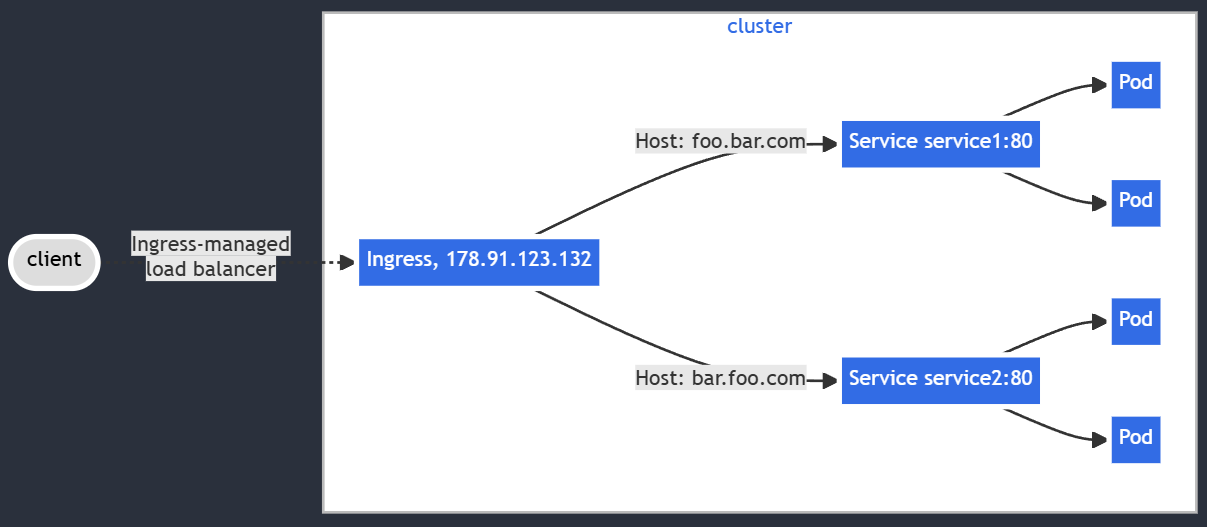
\includegraphics[width=\textwidth]{images/hChip/K8s/ingress-flow.png}
	\caption{Hình minh họa phân bố yêu cầu gọi đến các Service trong cụm ~\protect\footnotemark}
	\label{fig:k8s-ingress}
\end{figure}
\footnotetext{https://kubernetes.io/docs/concepts/services-networking/ingress/\#name-based-virtual-hosting}
\newpage
\subsection{RabbitMQ}
Đối với một hệ thống phân tán nói chung mà kiến trúc vi dịch vụ nói riêng, việc giao tiếp giữa các dịch vụ với nhau đóng vai trò then chốt.
Khác với các ứng dụng theo kiến trúc một khối (monolithic) truyền thống khi mà các thành phần giao tiếp với nhau thông qua các lời gọi hàm hoặc chia sẻ bộ nhớ, các ứng dụng theo kiến trúc vi dịch vụ giao tiếp với nhau qua hai hình thức chính~\footnote{https://learn.microsoft.com/en-us/dotnet/architecture/microservices/architect-microservice-container-applications/communication-in-microservice-architecture\#communication-types}:
\begin{itemize}
    \item Giao tiếp đồng bộ (Synchronous communication) là khi các dịch vụ gửi yêu cầu đến các dịch vụ đích và chờ phản hồi từ đó trước khi tiếp tục thực hiện tác vụ tiếp theo. Các giao thức phổ biến cho giao tiếp đồng bộ bao gồm RESTful API và gRPC (Remote Procedure Call).
    \item Giao tiếp bất đồng bộ (Asynchronous communication) khác với giao tiếp đồng bộ ở phương diện khi dịch vụ gửi yêu cầu không cần chờ phản hồi ngay lập tức từ các dịch vụ đích.
    Điều này cho phép dịch vụ tiếp tục thực hiện các tác vụ khác trong khi chờ phản hồi.
    Giao tiếp không đồng bộ thường được thực hiện thông qua việc sử dụng hàng chờ tin nhắn (message queue).
\end{itemize}
Việc chọn ra một chuẩn giao tiếp phù hợp với ứng dụng trong quá trình thiết kế mang ý nghĩa quan trọng khi mà mỗi cách giao tiếp đều đi kèm những lợi ích và giới hạn riêng cho từng hệ thống cũng như là đội phát triển ứng dụng.
Hệ thống quản lý quán ăn yêu cầu khả năng xử lý các yêu cầu từ khách hàng một cách nhanh chóng, hiệu quả, từ đó khi thiết kế hệ thống, hàng đợi tin nhắn như một lựa chọn tốt nhất với những yêu cầu nghiệp vụ nói trên.
Điều này giúp các dịch vụ giảm sự phụ thuộc vào nhau khi chỉ cần biết địa chỉ của hàng đợi tin nhắn mà không cần biết địa chỉ của các dịch vụ khác trong cùng mạng.
Hàng đợi tin nhắn cũng giúp tránh thất thoát dữ liệu, một trường hợp có thể xảy ra là khi một dịch vụ không hoạt động, các tin nhắn vẫn được lưu trữ ở trong hàng đợi và sẽ được xử lý một khi dịch vụ đó trở lại hoạt động.

Các công nghệ hàng đợi tin nhắn (message broker) phổ biến trên thị trường hiện nay có thể kể đến bao gồm Kafka, RabbitMQ, Amazon Simple Queue Service, v.v.
Ở đây, RabbitMQ được lựa chọn nhờ sự đơn giản trong quá trình triển khai và cài đặt đơn giản hơn các dịch vụ khác~\footnote{https://aws.amazon.com/compare/the-difference-between-rabbitmq-and-kafka/}.
Chi tiết về cách hàng đợi tin nhắn được sử dụng trong hệ thống quản lý quán ăn được đề cập ở Mục~\nameref{sec:system-architecture}.
\subsection{MongoDB}
Trong hệ thống quản lý nhà hàng phức tạp, việc lưu trữ và truy vấn dữ liệu hiệu quả là rất quan trọng.
Khác với các cơ sở dữ liệu truyền thống, MongoDB thuộc dạng cơ sở dữ liệu NoSQL, tức MongoDB có khả năng lưu trữ dữ liệu dạng tài liệu hay các dữ liệu phi cấu trúc một cách linh hoạt dưới dạng \tcode{BSON}~\footnote{https://www.mongodb.com/docs/manual/core/document/\#std-label-bson-document-format}. Điều này khiến cho cấu trúc bảng, dữ liệu có thể dễ dàng thích ứng với những thay đổi bất ngờ trong mô hình dữ liệu và yêu cầu nghiệp vụ.
Trong MongoDB, khái niệm khóa chính (primary key) và khóa ngoại (foreign key) không tồn tại theo cách hiểu truyền thống như trong các hệ quản trị cơ sở dữ liệu quan hệ (RDBMS). Tuy nhiên, MongoDB có những cơ chế riêng để đảm bảo tính toàn vẹn dữ liệu và tạo mối quan hệ giữa các bản ghi.
Đối với khóa chính, MongoDB tự động tạo một trường \tcode{\_id} cho mỗi tài liệu ngoại trừ những trường hợp người dùng chỉ định rõ~\footnote{https://www.mongodb.com/docs/manual/core/document/\#the-\_id-field}.
Trường này có giá trị là một \tcode{ObejctId} duy nhất trên toàn bộ cơ sở dữ liệu.
Giá trị của \tcode{ObejctId} là một chuỗi \tcode{byte} dài 12 ký tự trong đó 4 \tcode{byte} mang giá trị là thời gian tạo \tcode{Id}, 5 \tcode{byte} là giá trị ngẫu nhiên được tạo ra dựa theo \tcode{Id} của tiến trình và của máy, cuối cùng là 3 \tcode{byte} được tạo với một bộ đếm tăng dần, bộ đếm này sẽ được khởi tạo với một giá trị ngẫu nhiên~\footnote{https://www.mongodb.com/docs/manual/reference/method/ObjectId/}.

Ngoài ra, MongoDB còn có một phiên bản dịch vụ đám mây gọi là MongoDB Atlas, mang lại nhiều lợi ích như khả năng mở rộng tài nguyên tự động, sao lưu và phục hồi dữ liệu, giám sát và cảnh báo, giúp giảm thiểu công việc quản trị và đảm bảo hệ thống luôn sẵn sàng phục vụ.

\begin{figure}[h]
	\centering
	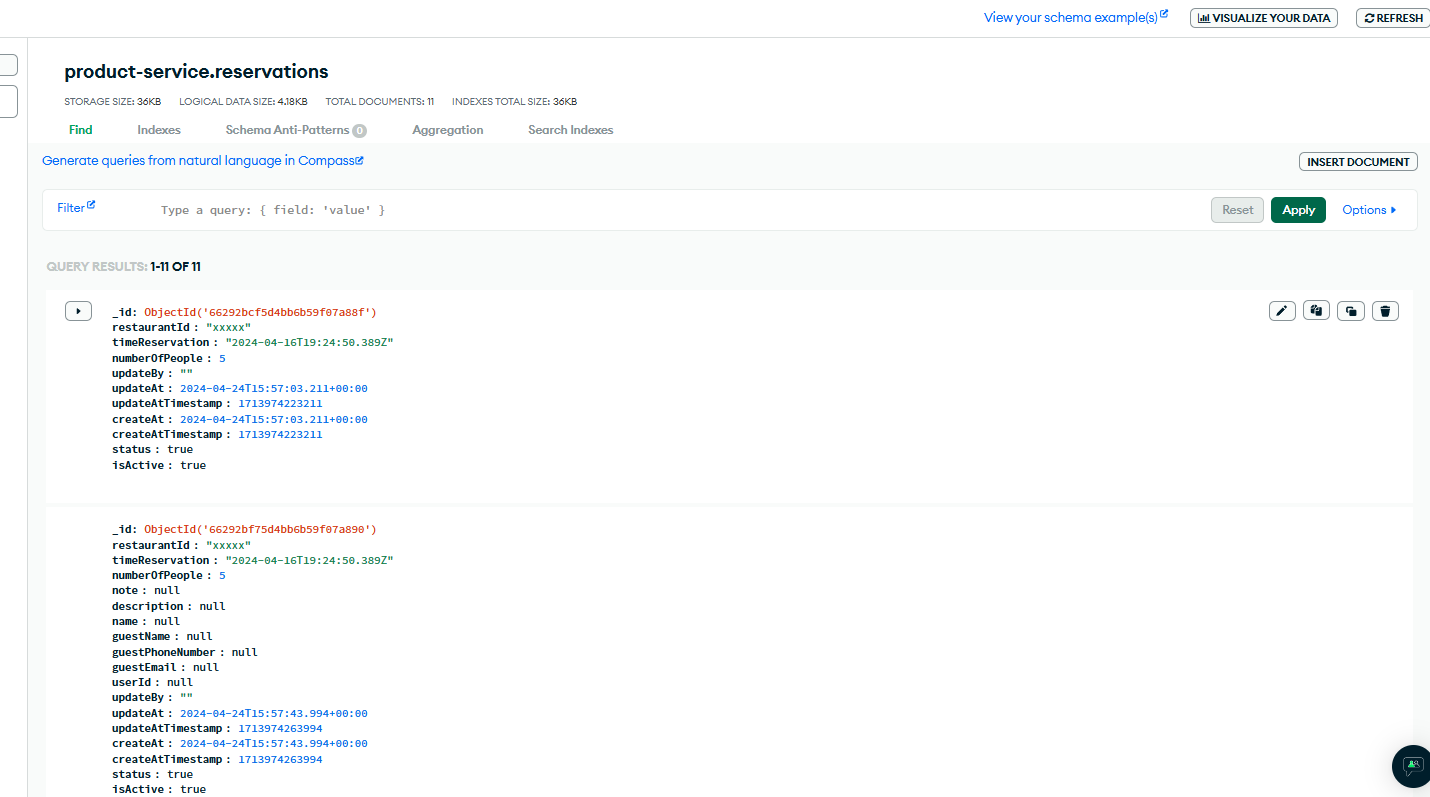
\includegraphics[width=\textwidth]{images/hChip/MongoDB/mongodb-preview.png}
	\caption{Giao diện người dùng của MongoDB Atlas}
	\label{fig:mongoDB-preview}
\end{figure}

Đối với một cơ sở dữ liệu thông thường, việc giám sát thông tin thường tập trung vào các loại như hiệu suất truy vấn, mức độ sử dụng tài nguyên, và trạng thái hoạt động.
Các chức năng này đều được MongoDB Atlas cung cấp trên nền tảng website gồm các chức năng như ghi nhật ký, các cảnh báo tùy chỉnh theo nhu cầu người dùng, giám sát tài nguyên hoạt động theo thời gian thực, v.v.
Từ đó khóa luận này quyết định sử dụng MongoDB cũng như là MongoDB Atlas làm cơ sở dữ liệu của hệ thống quản lý quán ăn.
Về chi tiết về mặt thiết kế cơ sở dữ liệu của hệ thống quản lý nhà hàng, quán ăn được đề cập ở Mục~\nameref{sec:database-design}.
\subsection{Kong}
Các hệ thống lớn hàng ngày sẽ phải tiếp nhận các lời gọi với tần suất rất lớn từ người dùng, đặc biệt là trong các giờ cao điểm trong ngày.
Không những thế, những hệ thống này còn có thể phải đối mặt với nguy cơ bị DDOS (Distributed Denial-of-Service), tức khi hệ thống bị ngợp bởi một lượng truy cập lớn có thể gây ra tê liệt hệ thống.
Cổng API (API Gateway) từ đây mang lại tác dụng như một điểm truy cập duy nhất cho ứng dụng, từ đó cấu hình chi tiết bên trong của nền tảng được ẩn dưới lớp API Gateway này.
Một trong những cổng API phổ biến đó là Kong Gateway.
Kong cung cấp các tiện ích khi sử dụng như chuyển đổi giao thức, đánh số, kiểm soát phiên bản API, giới hạn tốc độ truy cập và tích hợp các dịch vụ xác thực ở bên ngoài, v.v.

Khóa luận này thực hiện triển khai Kong Gateway trên một máy chủ thuộc GCP với Kong Manager.
Kiến trúc nền tảng của công gồm 3 thành phần bao gồm bộ định tuyển (router), dịch vụ (service), và máy chủ đích (upstream).
Khi nhận được yêu cầu từ ngoài vào, Kong Gateway sẽ khớp yêu cầu với Route phù hợp và chuyển tiếp yêu cầu đến Service tương ứng hoặc là tới các cân bằng tải đến cụm các Service trong Upstream.
Nhằm quản lý Kong dễn dàng và hiệu quả hơn, khóa luận sử dụng Kong Manager.
Kong Manager là bản thân Kong Gateway đã được trực quan hóa trên nền tảng web, điều này giúp người dùng dễ dàng tạo, chỉnh sửa và xóa các Route, Service và Upstream, phát triển, cấu hình các plugin nhằm mở rộng chức năng của Kong Gateway, giám sát lưu lượng truy cập API và hiệu suất của Kong.
\section{Quy trình triển khai}\label{sec:deploy-environment}
Trong bối cảnh phát triển các phần mềm hiện đại, khi mỗi dự án bao gồm nhiều đội ngũ phát triển phần mềm khác nhau với tần suất thay đổi mã nguồn ngày.
Nhằm lưu trữ, theo dõi các thay đổi một cách hiệu quả cũng như tăng cường hiệu quả phối hợp giữa các thành viên trong nhóm phát triển, các phần mềm quản lý mã nguồn (VCS - Version Control System) dần trở thành công cụ không thể thiếu trong giai đoạn phát triển cũng như là triển khai hệ thống.
Các VCS tiêu biểu có thể kể đến như là GitLab và GitHub, mặc dù cả hai nền tảng đều cung cấp đầy đủ các phương pháp quản lý mã nguồn hệ thống, cấu hình quyền người dùng linh hoạt và đều tích hợp các công cụ hỗ trợ kiểm thử hệ thống mạnh mẽ, GitLab nổi trội hơn GitHub về mặt tích hợp và triển khai liên tục (CI/CD) tốt hơn GitHub do cung cấp nhiều chức năng như bỏ qua các quy trình triển khai khi cần thiết, kết quả chạy đồng nhất và hiệu quả hơn, v.v. nên GitLab được lựa chọn là nền tảng quản lý mã nguồn cho hệ thống quản lý quán ăn.

Nền tảng quản lý quán ăn được chia làm tám kho lưu trữ mã nguồn (repository) bao gồm năm kho lưu trữ các mã nguồn thuộc về mặt logic của hệ thống, mỗi bộ mã nguồn tương dương với một vi dịch vụ và ba kho lưu trữ bao gồm trang giới thiệu (landing-page), trang quản lý nhà hàng (admin-page), và một trang mô phỏng phần đặt hàng của người dùng (customer-page).

Khi một thay đổi đối với mã nguồn được đẩy lên kho lưu trữ của GitLab, một quá trình kiểm tra và triển khai được cấu hình trước sẽ được chạy bởi GitLab Runner.
GitLab Runner là một ứng dụng chuyên biệt được phát triển bởi GitLab tích hợp với kho lưu trữ giúp chạy các câu lệnh cấu hình, kiểm thử và triển khai mã nguồn.
Ngoài lựa chọn sử dụng GitLab runner của riêng GitLab, việc tự triển khai riêng các GitLab Runner mang giúp khả năng tuỳ chỉnh cấu hình cụ thể của hạ tầng CI/CD, từ đó giúp tiết kiệm chi phí vận hành.

Có hai pha chính sẽ được thực hiện mỗi khi nhà phát triển phần mềm đẩy code lên kho mã nguồn của GitLab do GitLab Runner phụ trách đó là pha biên dịch mã nguồn và triển khai mã nguồn trên K8s và một pha phụ đó là cấu hình tệp \tcode{.env} cho mã nguồn trước đó giúp đẩy các biến môi trường giúp biên dịch mã nguồn.
Khi một thay đổi mới được đẩy lên GitLab, GitLab Runner sẽ tìm đọc tệp cấu hình \tcode{.gitlab-ci.yml} để xác nhận những chỉ dẫn cần được thực thi.

\begin{lstlisting}[style=yaml, caption={Đoạn mã cấu hình cài đặt biến môi trường cho GitLab Runner.}, label={cod:env-gitlab-ci/cd},  captionpos=b]
build_env:
  tags:
    - ${RUNNER_TAG}
  stage: build_env
  image: alpine/k8s:1.23.16
  script:
    - cat $PATH_DOCKER_BUILD_ENV_FILE > .env
  artifacts:
    paths:
      - .env
\end{lstlisting}

Đoạn mã~\ref{cod:env-gitlab-ci/cd} cho thấy cách đẩy tệp \tcode{.env} vào môi trường biên dịch.
Biến môi trường \tcode{\$PATH\_DOCKER\_BUILD\_ENV\_FILE} được sử dụng trong đoạn mã được cấu hình trong như một biến môi trường của dự án trên GitLab bên cạnh các biến môi trường khác được GitLab cung cấp sẵn khi chạy CI/CD.
Ở đây giá trị của biến là nội dung tệp \tcode{.env} là các biến hệ thống cần giúp cho hệ thống có thể biên dịch thành công bao gồm địa chỉ của kho lưu trữ ảnh và tệp trên Amazon S3, các biến trỏ đến đường dẫn các dịch vụ khác của hệ thống.

Sau khi mã nguồn trên kho lưu trữ của GitLab có tệp \tcode{env} cần thiết, GitLab Runner sẽ bắt đầu quá trình biên dịch mã nguồn hệ thống. Đoạn mã~\ref{cod:build-gitlab-ci/cd} sử dụng \tcode{kaniko} giúp chạy lệnh biên dịch mã nguồn sang ảnh Docker.
Kaniko~\footnote{https://github.com/GoogleContainerTools/kaniko} là một công cụ giúp xây dựng các ảnh Docker từ Dockerfile, có thể chạy bên trong một container hoặc một cụm K8s.
Kaniko giúp giải quyết hai vấn đề khi build Docker trong Docker (Docker-in-Docker)~\footnote{https://docs.gitlab.com/ee/ci/docker/using\_docker\_build.html\#use-docker-in-docker} đó là tránh việc phải chạy Docker ở quyền quản trị trong ảnh Docker, vốn là một điều phải có khi cần quyền truy cập vào Docker daemon của máy chủ, và giúp tối ưu quá trình chạy Docker-in-Docker (DinD) thông qua caching hiệu quả các lớp (layer) ảnh Docker~\footnote{https://cloud.google.com/blog/products/containers-kubernetes/introducing-kaniko-build-container-images-in-kubernetes-and-google-container-builder-even-without-root-access}.

\begin{lstlisting}[style=yaml, caption={Đoạn mã cấu hình quá trình biên dịch mã cho GitLab Runner.}, label={cod:build-gitlab-ci/cd},  captionpos=b]
build:
  stage: build
  tags:
    - ${RUNNER_TAG}
  image:
    name: gcr.io/kaniko-project/executor:debug
    entrypoint: [""]
  before_script:
    # - echo $IMAGE_REGISTRY_URL
    - echo $IMAGE_REGISTRY_USER
    # - echo $IMAGE_REGISTRY_PASS
    - echo "{\"auths\":{\"$IMAGE_REGISTRY_URL\":{\"auth\":\"$(printf "%s:%s" "$IMAGE_REGISTRY_USER" "$IMAGE_REGISTRY_PASS" | base64 | tr -d '\n')\"}}}" > /kaniko/.docker/config.json
    # - cat /kaniko/.docker/config.json
  script:
    - ls -la
    - cat .env
    - echo $IMAGE_NAME_BUILD
    - echo $IMAGE_NAME_BUILD_LATEST
    - /kaniko/executor
      --context "${CI_PROJECT_DIR}"
      --dockerfile "${CI_PROJECT_DIR}/Dockerfile"
      --cache=true
      --destination "$IMAGE_REGISTRY_URL/$IMAGE_NAME_BUILD_LATEST"
\end{lstlisting}

Trong Đoạn mã~\ref{cod:build-gitlab-ci/cd}, phần \tcode{before\_script} giúp người dùng đăng nhập vào một kho lưu trữ ảnh Docker (Docker Registry) giúp dễ dàng quản lý và triển khai trên K8s.
Sau đó GitLab Runner chạy phần \tcode{script} để biên dịch hệ thống dựa theo tệp \tcode{Dockerfile} được định nghĩa trước trong quá trình phát triển và kiểm thử hệ thống.

Cuối cùng pha triển khai (deploy) mã lên K8s của GCP, GitLab Runner được cấu hình chạy một tệp lệnh chương trình sử dụng kubectl, một công cụ giúp giao tiếp với các Master Node (Control Plane)~\footnote{https://kubernetes.io/docs/reference/kubectl/}.
Các cấu hình cho môi trường K8s nằm trong tệp \tcode{deployment-gke.yml} bao gồm các thành phần cài đặt cấu hình cho Ingress, Service và Deployment của hệ thống.
Đối với phần cấu hình cho Ingress và Service, K8s sẽ chỉ cần có số cổng mà ứng dụng mở ra ngoài và tên của kho mã nguồn, tuy nhiên ở phần cấu hình cho Deployment và autoscaling (tự động mở rộng), các trường thông tin sẽ ảnh hưởng nhiều đến hiệu năng của ứng dụng hơn như thông số của API kiểm tra tình trạng hoạt động, các thông số cấu hình phần cứng liên quan đến bộ nhớ và CPU cho mỗi Pod, và giới hạn số lượng pod tối đa khi hệ thống mở rộng cũng như là ngưỡng hệ thống quá tải cần mở rộng thêm.
\begin{lstlisting}[style=yaml, float,floatplacement=H,caption={Đoạn mã cấu hình cài đặt tự động mở rộng Kubernetes cho GitLab Runner.}, label={cod:k8s-gitlab-ci/cd},  captionpos=b, escapechar=|]
apiVersion: autoscaling/v2
kind: HorizontalPodAutoscaler
metadata:
  name: $CI_PROJECT_NAME
  namespace: $CI_PROJECT_ROOT_NAMESPACE
spec:
  scaleTargetRef:
    apiVersion: apps/v1
    kind: Deployment
    name: $CI_PROJECT_NAME
  minReplicas: 1
  maxReplicas: 5|\label{line:sp}|
  metrics:
    - resource:
        name: memory
        target:
          averageUtilization: 80
          type: Utilization
      type: Resource
    - resource:
        name: cpu
        target:
          averageUtilization: 50
          type: Utilization
      type: Resource
\end{lstlisting}
Nhằm phục vụ quá trình kiểm thử sản phẩm ở Chương~\nameref{chap4}, ngưỡng tự động mở rộng trong Đoạn mã~\ref{cod:k8s-gitlab-ci/cd} được đặt tại giới hạn sử dụng 80\% bộ nhớ và 50\% CPU.
Khi bất kỳ một Pod nào thuộc Deployment đạt tới ngưỡng, GKE sẽ tự động tạo thêm một Pod mới giúp giãn tải trên các Pod đang hoạt động, tới một giới hạn số lượng Pod tối đa là năm như được cấu hình tại Dòng~\ref{line:sp}, Đoạn mã~\ref{cod:k8s-gitlab-ci/cd}.
\section{Một số luồng chức năng chính}\label{sec:user-flow-examples}
Như đã nói ở Mục~\ref{sec:main-functions}, các luồng chính của nền tảng quản lý nhà hàng, quán ăn được mô tả sẽ bao gồm luồng đặt bàn của người dùng khách hàng tại quán ăn và luồng đặt đồ ăn thông qua việc quét mã QR từ phía người dùng.
Ở Chương này, ta sẽ đi sâu vào luồng di chuyển của người dùng cũng như là các lời gọi dữ liệu giữa các dịch vụ với nhau trong hệ thống.
\subsection{Luồng đặt bàn}\label{sec:reservation-sequence-flow}
Sơ đồ tuần tự ở Hình~\ref{fig:reservation-sequence-flow} mô tả cách người dùng tương tác với tính năng đặt hàng trên giao diện tại trang giới thiệu.
Sơ đồ tồn tại các tác nhân chính là người dùng/thực khách có nhu cầu đặt bàn, giao diện người dùng tương tác khi đặt bàn có thể từ trang giới thiệu nền tảng quản lý nhà hàng, quán ăn hoặc các trang riêng của nhà hàng có liên kết với hệ thống quản lý.
Tiếp theo đó là \tcode{product-service} tiếp nhận các lời gọi từ phía người dùng và xử lý chúng.
Hai tác nhân cuối gồm \tcode{admin-page} và nhân viên của cửa hàng phụ trách việc tiếp nhận, xác nhận lại yêu cầu đặt bàn của người dùng.

\begin{figure}[h]
	\centering
	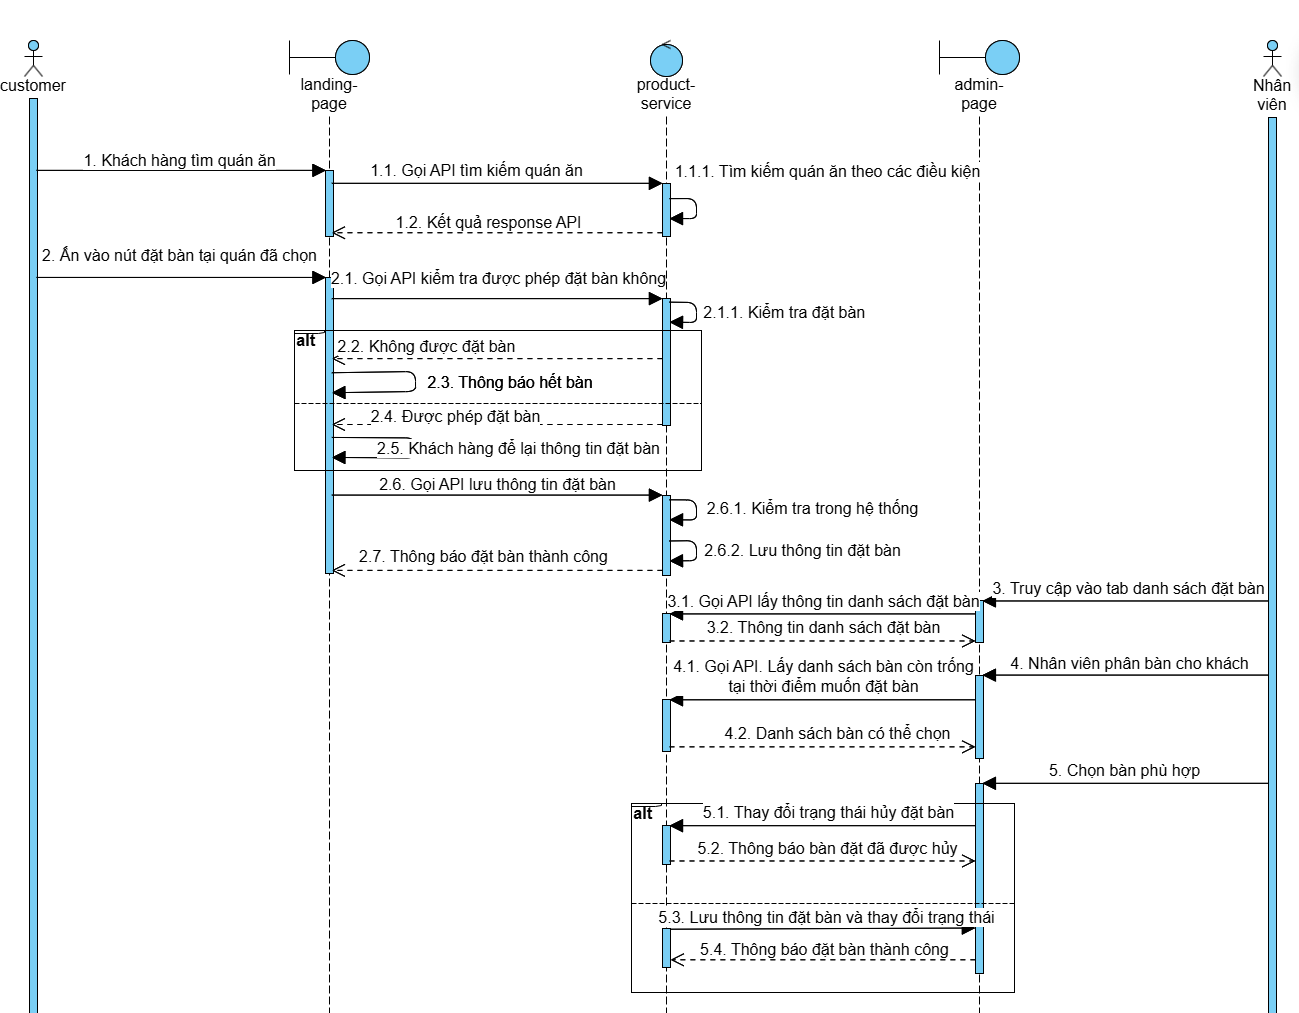
\includegraphics[width=\textwidth]{images/hChip/main-flow/reservation.png}
	\caption{Sơ đồ tuần tự mô tả luồng nghiệp vụ đặt bàn trực tuyến}
	\label{fig:reservation-sequence-flow}
\end{figure}

Luồng người dùng bắt đầu khi người dùng thực hiện tìm kiếm quán ăn trên trang giới thiệu của hệ thống hoặc của từng cửa hàng, khách hàng sẽ có lựa chọn đặt bàn tại quán ăn.
Sau khi khách hàng đã chọn xong bàn và điền các thông tin được yêu cầu, hệ thống sẽ kiểm tra tình trạng hiện tại của quán ăn và xác nhận lại với khách hàng tình trạng đặt bàn trên giao diện.
Một khi người dùng thực hiện đặt bàn thành công, thông tin sẽ được đẩy đến trung tâm thông báo và chuyển tiếp đến các dịch vụ khác, ở đây là trang quản lý nhà hàng. 
Nhân viên của quán ăn sẽ xác nhận yêu cầu đặt bàn của khách hàng và tiến hành phân bàn cho khách dựa trên số lượng, yêu cầu khi đặt bàn.
Nếu không thể chọn được bàn phù hợp cho yêu cầu của thực khách, nhân viên của quán ăn sẽ thay đổi trạng thái của phần đặt bàn thành đã hủy và ngược lại là thành công nếu có bàn.

Ở Hình~\ref{fig:reservation-sequence-flow} không có luồng thông báo cho người dùng về trạng thái đặt bàn do người đặt bàn có thể chưa đăng ký tham gia hệ thống, điều đó khiến cho việc thông báo cho người dùng trở nên khó khăn bởi hệ thống thông báo sẽ không biết thông tin của người dùng để hiển thị.
Nhân viên của quán sau khi thay đổi trạng thái của yêu cầu đặt bàn sẽ cần xác nhận, thông tin tới khách hàng theo dựa theo biểu mẫu mà khách cung cấp khi yêu cầu đặt bàn trên website.
\subsection{Luồng gọi món}\label{sec:order-sequence-flow}
Khi nhà hàng, quán ăn tham gia vào hệ thống quản lý sẽ được hỗ trợ tạo QR gán cho mỗi bàn thuộc nhà hàng giúp khách hàng có thể gọi món mà không cần tương tác với nhân viên của quán.
Hình~\ref{fig:order-sequence-flow} mô tả quá trình từ lúc người dùng sử dụng mã QR để đặt món và nhân viên, phục vụ của nhà hàng, quán ăn thay đổi trạng thái của đơn gọi món.
Các tác nhân trong sơ đồ bao gồm người dùng và nhân viên là hai tác nhân chính tương tác với hệ thống, trang \tcode{customer-page} giúp người dùng tương tác và thực hiện lời gọi đến hệ thống.
Các tác nhân đảm nhiệm việc xử lý bao gồm \tcode{order-service}, \tcode{product-service}, và \tcode{notification-service}.

\begin{figure}[h]
	\centering
	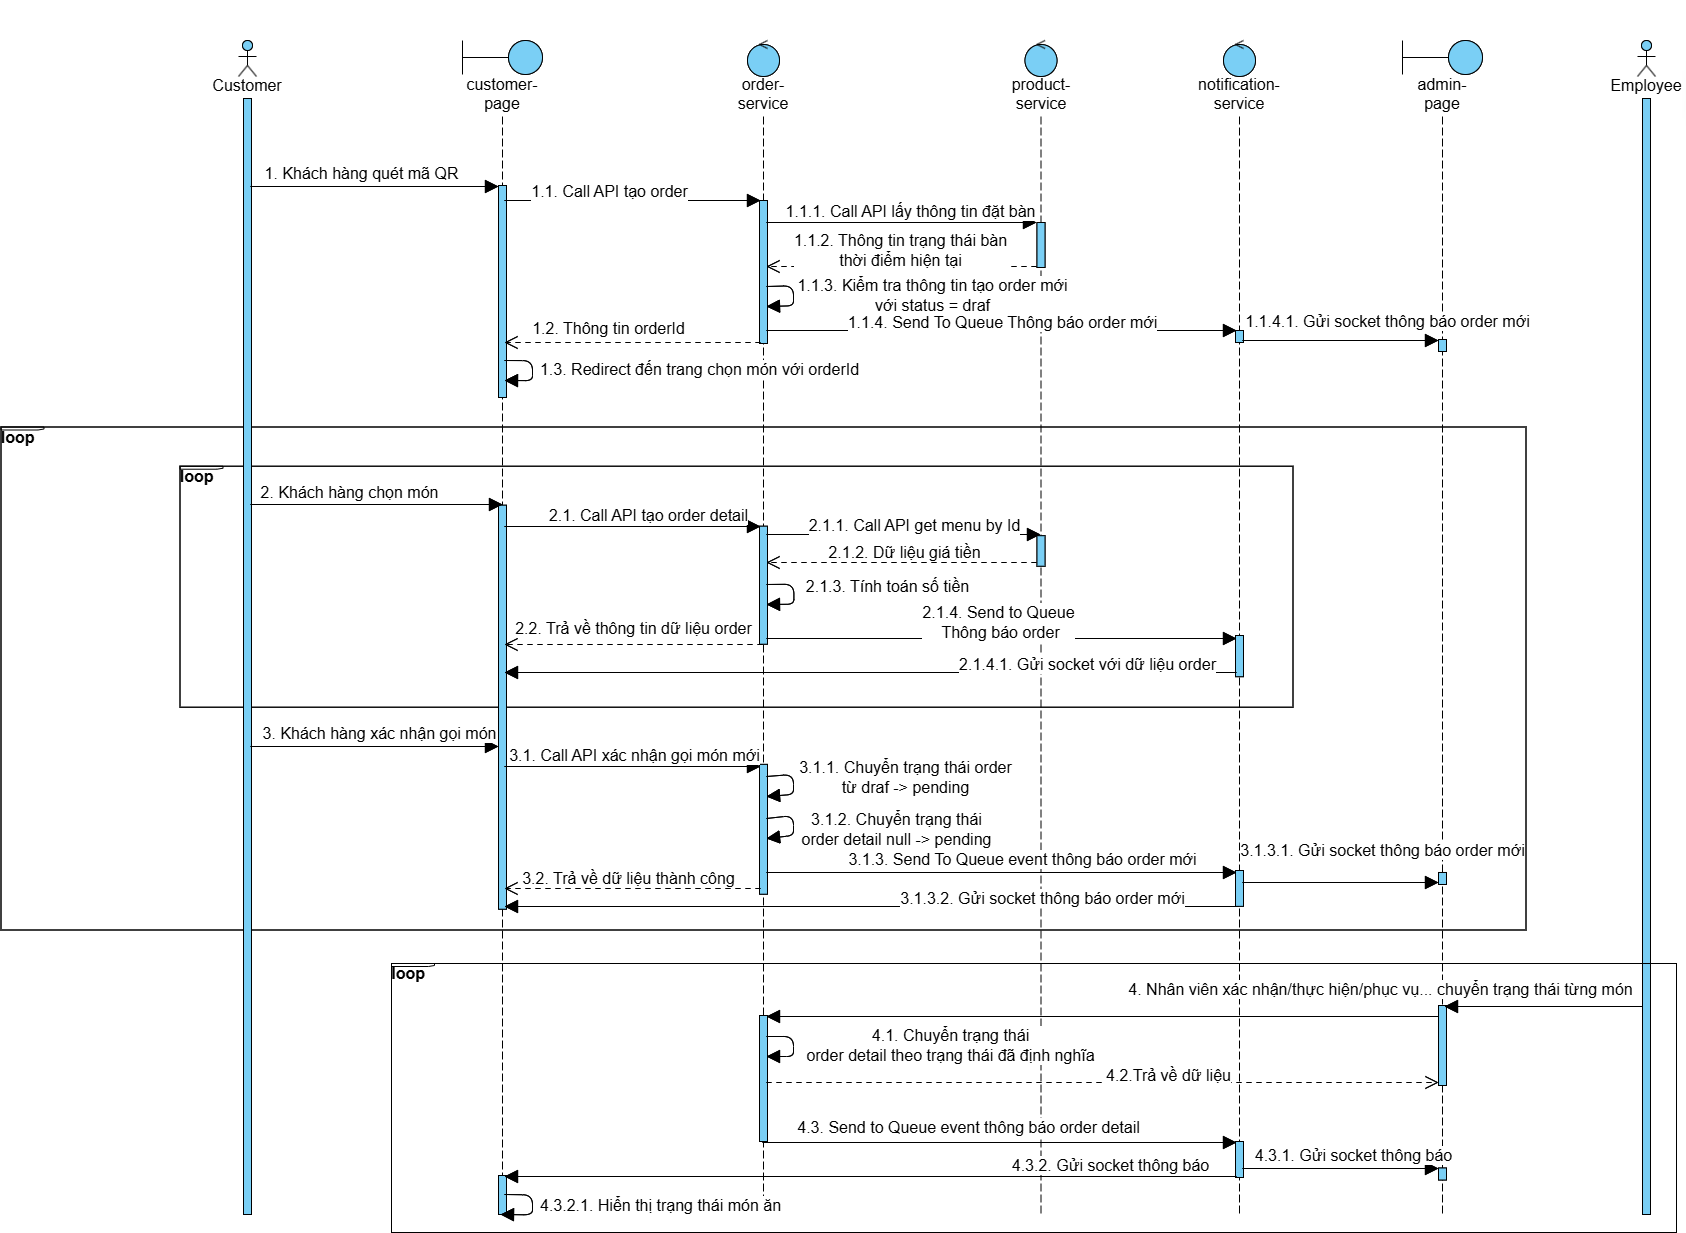
\includegraphics[width=1.1\textwidth]{images/hChip/main-flow/order.png}
	\caption{Sơ đồ tuần tự mô tả luồng nghiệp vụ đặt món thông qua quét mã QR}
	\label{fig:order-sequence-flow}
\end{figure}

Sau khi người dùng thực hiện quét mã QR, hệ thống sẽ thực hiện xác nhận tạo order mới cho số bàn đang ngồi với trạng thái là \tcode{draf}.
Khách hàng sẽ được chuyển hướng đến trang chọn món sau khi nhận lại \tcode{orderId}, ở đấy khách hàng sẽ chọn các món ăn từ thực đơn của quán.
Sau khi người dùng hoàn thành quá trình chọn đồ ăn cũng như xác nhận danh sách các món ăn cho đơn hàng, nhân viên, phục vụ, đầu bếp, v.v. sẽ chuyển trạng thái từng món cụ thể dựa theo tình trạng hiện tại của món ăn như \textit{đang chuẩn bị}, \textit{dã xong}, \textit{đã phục vụ}, v.v.
Toàn bộ luồng nghiệp vụ sẽ lặp lại cho đến khi người dùng chọn tính năng thanh toán và hoàn thành bữa ăn.
% \begin{table}[h]
%     \centering
%     \caption{Kết quả thời gian chuẩn bị môi trường trên ba mô-đun thực nghiệm}
%     \label{tab:time_undef}
% \begin{tabular}{|l|l|l|l|ll|}
% \hline
% \multicolumn{1}{|c|}{\multirow{2}{*}{\textbf{Module}}} & \multicolumn{1}{c|}{\multirow{2}{*}{\textbf{File}}} & \multicolumn{1}{c|}{\multirow{2}{*}{\textbf{Undef}}} & \multirow{2}{*}{\textbf{Compilable}} & \multicolumn{2}{c|}{\textbf{Linkable}} \\ \cline{5-6} 
% \multicolumn{1}{|c|}{}                                 & \multicolumn{1}{c|}{}                               & \multicolumn{1}{c|}{}                                &                                      & \multicolumn{1}{l|}{Manual}  & Propose \\ \hline
% collision (Box2d)                                      & 53                                                  & 5                                                    & 0:02:39                              & \multicolumn{1}{l|}{0:08:23} & 0:00:04 \\ \hline
% FPT1                                     & 45                                                  & 263                                                  & 1:04:22                              & \multicolumn{1}{l|}{0:14:48} & 0:00:28 \\ \hline
% FPT2                                          & 126                                                 & 333                                                  & 2:05:56                              & \multicolumn{1}{l|}{1:31:01} & 0:02:24 \\ \hline
% \end{tabular}
% \end{table}      
\chapter{Đánh giá hệ thống}\label{chap4}
Việc thực hiện đánh giá hệ thống sau khi đã triển khai trên môi trường thực nghiệm là một bước quan trọng giúp đảm bảo hệ thống hoạt động đúng như mong đợi, đáp ứng các yêu cầu về hiệu suất độ tin cậy và khả năng mở rộng.
Chương này sẽ đánh giá hiệu quả hoạt động thông qua các bộ kiểm thử được cấu hình sẵn.
Ngoài ra ở Chương này đề cập đến một số vấn đề gặp phải trong quá trình phát triển nên tảng quản lý quán ăn.
\section{Hiệu quả hoạt động}\label{sec:efficiency}
Để đánh giá hiệu quả hoạt động của hệ thống một cách toàn diện, hai bộ kiểm thử được tiến hành gồm kiểm thử tự động mở rộng và kiểm thử tính sẵn sàng cao.
Kiểm thử tự động mở rộng tập trung vào khả năng GKE tự động điều chỉnh tài nguyên, số lượng Node, Pod để đáp ứng với sự biến động trong lưu lượng truy cập.
Kiểm thử tính sẵn sàng cao sẽ đánh giá xem liệu hệ thống có thể duy trì hoạt động liên tục ngay cả khi gặp sự cố
\subsection{Kiểm thử tự động mở rộng}
Bằng việc sử dụng HPA của K8s trên môi trường đám mây của GCP, cấu hình phần cứng của các Pod được định nghĩa ở Đoạn mã~\ref{cod:storage-service-hardware}.
\tcode{limits} là cấu hình phần cứng tối đa (bộ nhớ và CPU) mà Pod đó được phép tiêu thụ.
Đây là giá trị ngưỡng cố định được đặt ra bởi K8s.
\tcode{requests} là số lượng bộ nhớ và CPU tối thiểu mà Pod yêu cầu để hoạt động và K8s sẽ đảm bảo lượng tài nguyên này sẽ luôn khả dụng cho Pod.
Theo cấu hình tại Dòng~\ref{line:sp}, Đoạn mã~\ref{cod:k8s-gitlab-ci/cd}, mỗi deployment sẽ có tối đa năm Pod hoạt động cùng lúc nhưng để phục vụ mục đích kiểm thử với lưu lượng thực tế của một hệ thống lớn, số lượng Pod tối đa đã được điều chỉnh lên 20 Pod.
Dịch vụ được chọn để chạy kiểm thử sẽ là dịch vụ lưu trữ tệp \tcode{storage-service}, dịch vụ này phụ trách việc lưu trữ ảnh và các tệp do người dùng tải lên một S3 bucket của AWS (Amazon Web Service).
API được gọi cho mục đích kiểm thử sẽ là một API lấy mã QR thanh toán của nhà hàng đã được tải lên S3.
\begin{lstlisting}[style=yaml, caption={Đoạn mã cấu hình phần cứng cho \tcode{storage-service} trên GKE.}, label={cod:storage-service-hardware},  captionpos=b]
resources:
    limits:
        cpu: 300m
        memory: 500Mi
    requests:
        cpu: 200m
        memory: 300Mi
\end{lstlisting}
\begin{figure}
    \centering
    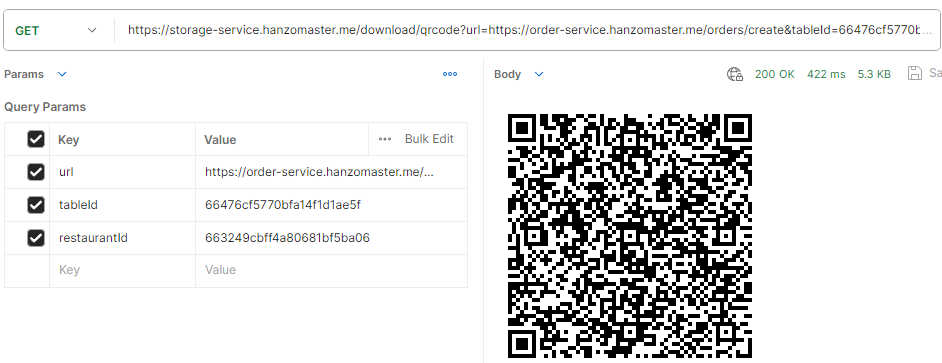
\includegraphics[width=1\linewidth]{images/hChip/test/API-example.png}
    \caption{API lấy mã QR thanh toán của nhà hàng, quán ăn}
    \label{fig:API-QR-code}
\end{figure}
\begin{figure}[H]
	\centering
	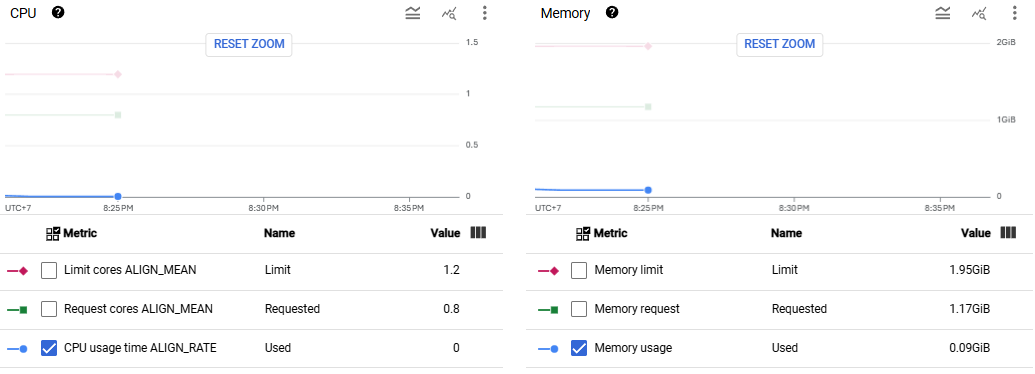
\includegraphics[width=\textwidth]{images/hChip/test/resourse-before-test.png}
	\caption{Lượng tài nguyên trước khi bắt đầu kiểm thử tự động mở rộng}
	\label{fig:resource-before-test}
\end{figure}
Hình~\ref{fig:resource-before-test} cho thấy lượng tài nguyên Deployment trước khi bắt đầu gọi API có số lượng bộ nhớ tối đa có thể truy cập được là \tcode{1.95GiB} tương đương với 4 Pod đang hoạt động.
Công cụ được sử dụng để chạy kiểm thử là Jmeter, một công cụ kiểm thử hiệu năng mã nguồn mở nổi tiếng thường xuyên được dùng trong các công việc liên quan đến đo lường và phân tích hiệu suất của cá ứng dụng web cũng như là các dịch vụ.
\begin{figure}
    \centering
    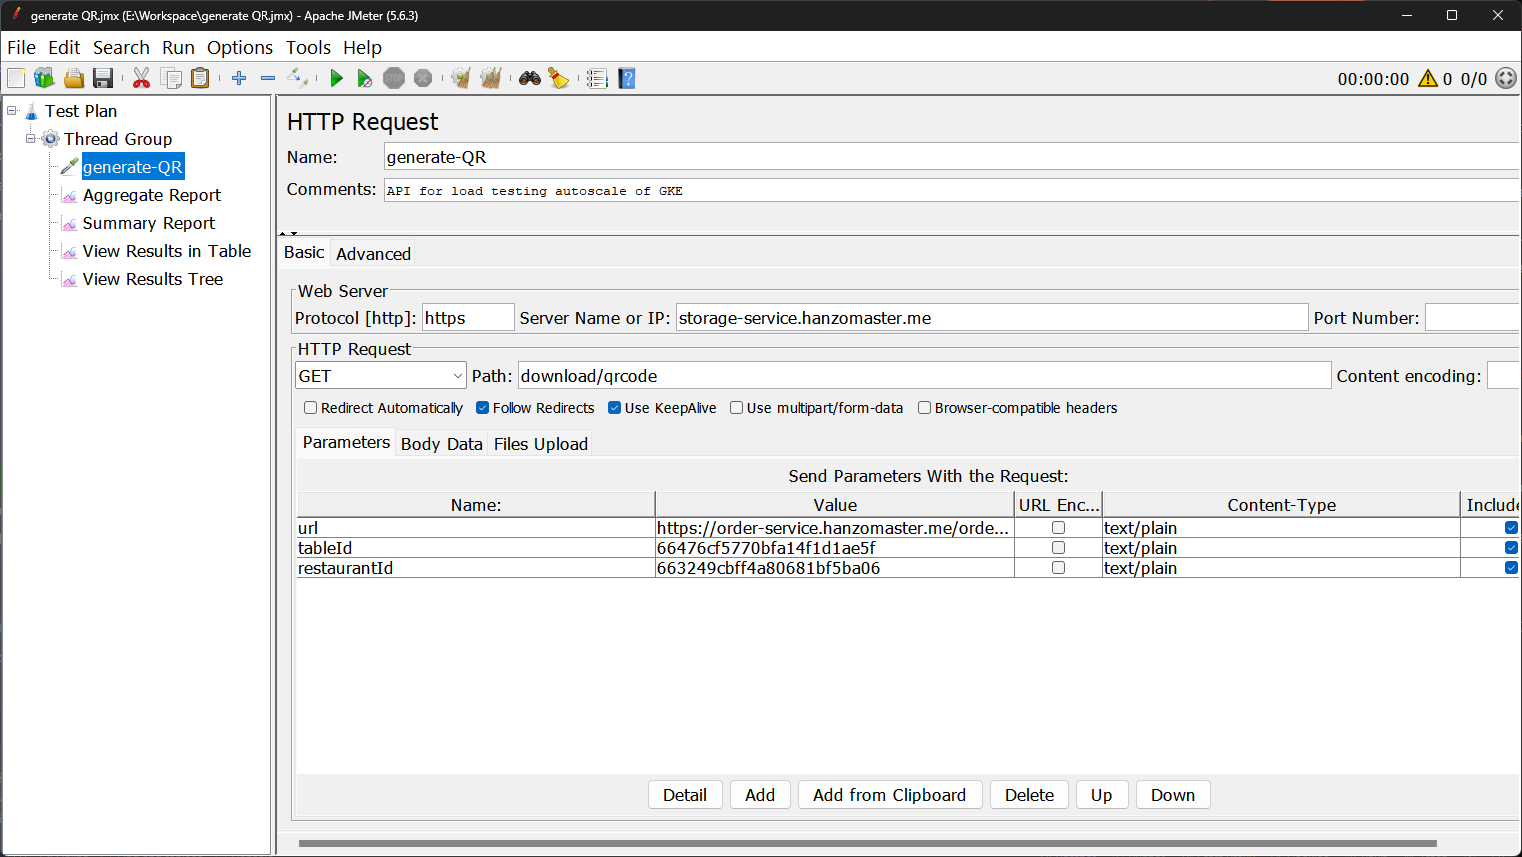
\includegraphics[width=1\linewidth]{images/hChip/test/Jmeter-setup.png}
    \caption{Bộ kiểm thử API của Jmeter}
    \label{fig:Jmeter-API}
\end{figure}
Cấu hình Jmeter chạy bộ kiểm thử API với 200 luồng tương đương với 200 người dùng và thời gian tăng trưởng (ramp-up period) 20 giây trong 15 phút, ta có được các chỉ số như sau.
\begin{figure}
    \centering
    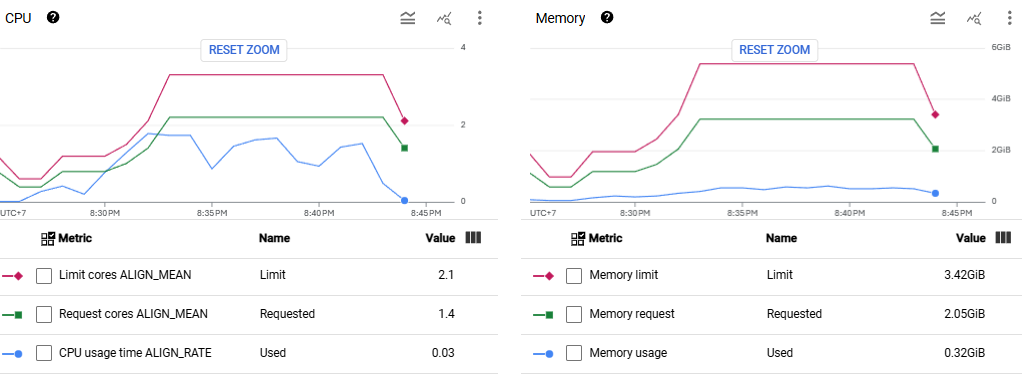
\includegraphics[width=1\linewidth]{images/hChip/test/resource-after-15m.png}
    \caption{Lượng tài nguyên sử dụng trong quá trình chạy Jemter kiểm tra tải}
    \label{fig:resource-after-15}
\end{figure}
Ở thời điểm số lượng lời gọi vào hệ thống nhiều nhất, hệ thống mở rộng lên tới 11 Pod và lượng tài nguyên được các Pod yêu cầu tiêu thụ là\tcode{3.22GiB}.
\begin{figure}
    \centering
    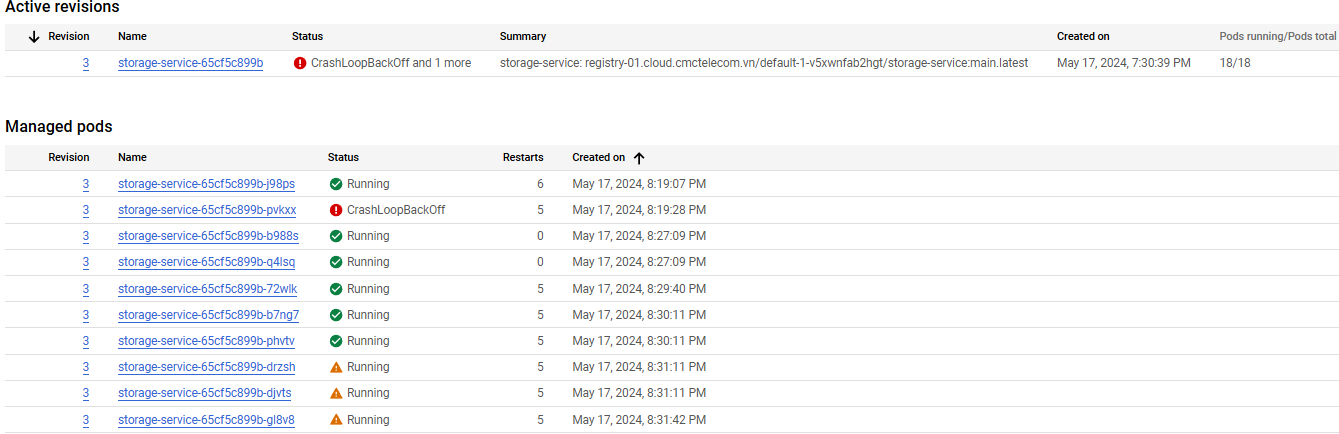
\includegraphics[width=1\linewidth]{images/hChip/test/pod-number-after-15m.png}
    \caption{Số lượng Pod trong quá trình chạy Jmeter kiểm tra tải}
    \label{fig:pod-number-after-15}
\end{figure}
Ngoài ra số lượng Node cũng được K8s cấu hình tăng cường lên trong quá trình này.
Một số Pod khi hệ thống hứng chịu một lượng yêu cầu lớn có biểu hiện lỗi do Pod dùng quá bộ nhớ giới hạn của K8s khiến cho Pod bị buộc tắt đi và bật lại.
Sau khi quá trình chạy Jmeter hoàn tất, các Pod đều trở lại hoạt động bình thường và K8s tự động giảm số lượng Node và Pod về cấu hình mặc định.
\subsection{Kiểm thử tính sẵn sàng cao}
Bộ kiểm thử này được sử dụng với mục tiêu xác định khả năng phục hồi của hệ thống khi gặp sự cố cũng như là tính sẵn sàng cao của hệ thống, tức khi một hệ thống không hoạt động thì các lời gọi yêu cầu đến vẫn có thể được xử lý tại một mức nhất định.
Có nhiều cách nhằm đảm bảo tính sẵn sàng cao của hệ thống, các phương pháp truyền thống vẫn hay được sử dụng như DC/DR (Data Center/Diaster Recovery) kèm theo cân bằng tải giúp giảm thiểu rủi ro khi một thành phần gặp sự cố.
Ngoài ra, việc sao lưu dữ liệu thường xuyên cũng là những biện pháp cần thiết giúp duy trì tính liên tục của dịch vụ.

Trong kiến trúc vi dịch vụ, việc sử dụng nhiều cụm K8s đã trở thành một giải pháp hiệu quả để duy trì HA.
Với cách tiếp cận này, ứng dụng sẽ được triển khai trên nhiều cụm K8s độc lập, phân tán trên các vùng địa lý khác nhau.
Khi một cụm gặp sự cố, lưu lượng truy cập sẽ được tự động chuyển hướng đến các cụm khác, đảm bảo tính liên tục của dịch vụ.
Trên thực tế, việc duy trì tính liên tục của hệ thống còn gặp nhiều khó khăn do vấn đề không chỉ nằm ở cụm K8s chạy các dịch vụ xử lý chính của hệ thống mà lỗi có thể rải rác ở bất cứ vị trí nào từ Cổng API, cân bằng tải của Clouflare, cơ sở dữ liệu MongoDB.
Ở mỗi vùng này ta đều cần có các biện pháp sao lưu, dự phòng phù hợp giúp tránh hệ thống gặp sự cố khiến cho dịch vụ ngừng hoạt động.

Hệ thống quản lý nhà hàng, quán ăn được cấu hình chia làm hai cụm chạy độc lập với nhau trên GKE của GCP.
Từ đó ta sẽ cấu hình Cổng API của Kong giúp cân bằng tải đến cả hai cụm.
Ở đây ta sẽ điều chỉnh thêm một Upstream mới với IP của máy chủ đích đến là cụm dự phòng của hệ thống với cùng một thông số \tcode{Weight}.
Điều này có nghĩa là lưu lượng truy cập sẽ được phân phối điều cho cả hai máy chủ.
\begin{figure}[H]
    \centering
    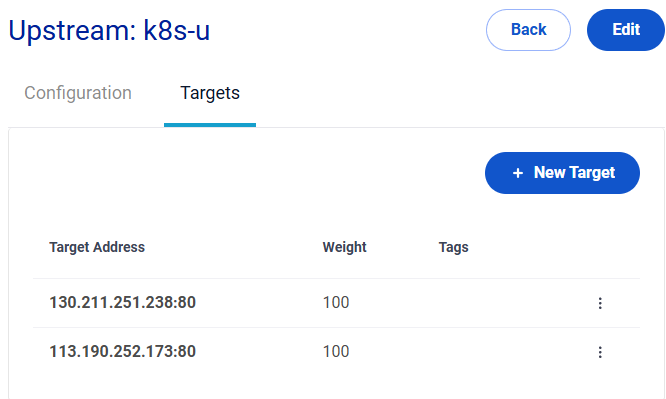
\includegraphics[width=1\linewidth]{images/hChip/test/kong-upstream.png}
    \caption{Các máy chủ được cấu hình trỏ đến trong Kong Gateway}
    \label{fig:kong-upstream}
\end{figure}
Sau khi đã cấu hình xong, giờ đây thông qua các API kiểm tra tình trạng của hệ thống (health check), Kong Gateway sẽ định kỳ gọi đến các API này nhằm phát hiện hệ thống có gặp phải sự cố hay không.
Khi một hệ thống bị đánh dấu là ngừng hoạt động, Kong Gateway sẽ ngừng chuyển hướng lưu lượng truy cập máy chủ đó mà chuyển các yêu cầu gọi API đến máy chủ còn đang hoạt động.
Khi máy chủ gặp sự cố nhận yêu cầu gọi trở lại, Kong Gateway sẽ tự động phát hiện thông qua API kiểm tra tình trạng hoạt động của hệ thống và chuyển hướng lưu lượng truy cập trở lại máy chủ đó.
Điều này giúp ứng dụng đạt tính sẵn sàng cao khi hạn chế được thời gian ngừng hoạt động của hệ thống bằng cách phân phối dữ liệu trên nhiều máy chủ khác nhau.
\chapter*{Kết luận}\label{chap5}
\addcontentsline{toc}{chapter}{Kết luận}
Khóa luận này đã trình bày chi tiết về quá trình nghiên cứu, thiết kế, và triển khai một hệ thống quản lý nhà hàng toàn diện, đáp ứng nhu cầu của cả chủ nhà hàng và khách hàng.
Hệ thống không chỉ cung cấp các công cụ quản lý hiệu quả cho nhà hàng, quán ăn mà còn tạo ra một nền tảng tương tác thuận tiện cho khách hàng thông qua các tính năng đặt bàn trực tuyến và đặt món trực tuyến thông qua quét mã QR và quản lý thông tin cá nhân.

Việc áp dụng kiến trúc vi dịch vụ cùng với việc tận dụng khả năng mở rộng tự động của GKE đã giúp hệ thống đạt được tính linh hoạt, khả năng chịu lỗi cao và khả năng đáp ứng nhu cầu sử dụng biến động. Các bộ kiểm thử đã chứng minh hiệu quả hoạt động của hệ thống trong việc tự động mở rộng và duy trì tính sẵn sàng cao, đảm bảo trải nghiệm người dùng mượt mà và không bị gián đoạn.

Tuy còn một vài hạn chế trong thiết kế và tích hợp hoàn chỉnh các luồng nghiệp vụ của hệ thống, sau khi các vấn đề được khắc phục trong tương lai gần, hệ thống sẽ tiếp tục được mở rộng và phát triển với các tính năng mới nhằm nâng cao trải nghiệm người dùng và đáp ứng tốt hơn nhu cầu thị trường.
Một số các chức năng trong số đó ao gồm tính năng đặt món trực tuyến trên trang giới thiệu của nhà hàng, quán ăn, quản lý chế độ dinh dưỡng của người dùng, gợi ý món ăn tại trang đặt món, phát triển ứng dụng di động, v.v.

Bên cạnh đó, ứng dụng hoàn toàn có tiềm năng tận dụng những dữ liệu từ cửa hàng cũng như là khách hàng sử dụng nền tảng để áp dụng công nghệ trí tuệ nhân tạo (AI) nhằm phát triển các chức năng đột phá mới.
Ví dụ, AI có thể được sử dụng để phân tích dữ liệu của người dùng, từ đó đưa ra các gợi ý món ăn tùy biến theo các thông tin thu thập được.
Hoặc AI giúp dự đoán xu hướng ẩm thực và hỗ trợ nhà hàng trong việc xây dựng chiến lược kinh doanh hiệu quả.

Với những định hướng phát triển này, hệ thống quản lý nhà hàng được kỳ vọng sẽ đóng góp tích cực vào sự phát triển của ngành dịch vụ ăn uống tại Việt Nam, giúp các nhà hàng tối ưu hóa quy trình quản lý, nâng cao chất lượng dịch vụ và tăng cường khả năng cạnh tranh trên thị trường.
Với sự phát triển không ngừng của công nghệ, hệ thống này sẽ tiếp tục được cải tiến và hoàn thiện, mang đến những giải pháp tiên tiến và hiệu quả hơn cho ngành công nghiệp này.

\chapter*{Tài liệu tham khảo}
\addcontentsline{toc}{chapter}{Tài liệu tham khảo}
\printbibliography[keyword={vietnam}, heading=subbibliography, title={Tiếng Việt}, resetnumbers=true]
\printbibliography[notkeyword={vietnam}, heading=subbibliography, title=Tiếng Anh]
\end{document}